\documentclass[11pt,letterpaper,twoside]{article}
\usepackage[tmargin=1in,bmargin=1in,lmargin=1in,rmargin=1in]{geometry}
\usepackage{../style/packages}
\usepackage{../style/commands}
\setbool{notesonly}{false}

% -------------------
% Content
% -------------------
\begin{document}

% Cover Photo
% !TEX root = ../main/aws_perfectoid.tex

\thispagestyle{empty}
\newgeometry{
	top=0cm, 
	bottom=0cm, 
	left=0cm, 
	right=0cm
}


\tikz[remember picture,overlay] \node[opacity=1,inner sep=0pt] at (current page.center){
\includegraphics[width=\paperwidth,height=\paperheight]{../cover/swc_poster.jpg}};

\phantom{x} % To image is placed.

% Reset Page Style
\newgeometry{
	top= 1in, 
	bottom= 1in, 
	left= 1in, 
	right= 1in
}
\newpage

% Cover
% !TEX root = ../main/aws_perfectoid.tex

\thispagestyle{empty}
\begin{flushright}
\begin{tabular}{ll}
\raisebox{-.5\height}{
\includegraphics[scale=0.055]{../cover/arizona_seal.png}} & {\color{ArzBlue} \Huge University of Arizona} 
\end{tabular}
\end{flushright}
\vspace{2in}

{%
\color{ArzRed} \Huge \noindent Arizona Winter School 2017 \par \Huge \noindent \color{ArzRed} Perfectoid Spaces \par \color{ArzBlue}
\noindent \rule{0.70\textwidth}{0.05cm}
}

{\color{ArzBlue} \large \noindent Notes By: Caleb McWhorter }

\vfill
\begin{center} {\color{ArzBlue}\huge March 2017} \end{center}
\newpage

% TOC
\thispagestyle{blank}
\tableofcontents
\newpage

% -------------------
% Lectures
% -------------------

% Lecture Notes
\thispagestyle{empty}
\part{Talk Notes} 
    \newpage 
	\setcounter{page}{1}

% Scholze
% !TEX root = ../../../main/aws_perfectoid.tex
\newpage
\section{Name: Lecture Title}
\subsection{Lecture 1}
\subsubsection{Lecture Name}

Historic Remarks about the genesis of the paper ``Perfectoid Spaces''

or why perfectoid spaces are a failed theory.

In 2007, Scholze went to Bonn as an undergrad and studied under M. Rapport. 


Let $X$ be a smooth projective scheme over $\Q_p$. Fix $i \geq 0$ and let $l \neq p$ be a prime. Consider the $\Gal(\ov{\Q}_p/\Q_p)$-representation $V= H_\et^i(X_{\ov{\Q}_p}, \ov{\Q}_l)$. There is a weight decomposition given by the following: if $\Phi \in \Gal(\ov{\Q}_p/\Q_p)$ is a geometric Frobenius, then 
	\[
	V= \bigoplus_{j=0}^{2i} V_j,
	\]
where $\Phi$ acts through the Weil numbers of weight $j$ on $V_j$. 


Rapport-Zink (1980) if $X$ has semistable reduction 

de Joung (1995) in general (reduction to semistable case).


Rapport gave Scholze the following problem to think about:

There is a monodromy operator $N: V \to V(\pm 1)$ (Tate twist) coming from the action of the inertia subgroup. In particular, $N: V_j \to V_{j-2}$. Then
	\[
	\forall j=0,\ldots,i: N^j: V_{i+j} \ma{\sim} V_{i-j}.
	\]









\begin{conj}[Weight-Monodromy Conjecture]
Let $X$ be a smooth projective scheme over $\Q_p$. Fix $n \geq 0$ and $l \neq p$ a prime. Consider the $\Gal(\ov{\Q}_p/\Q_p)$-representation $V= H_\et^i(X_{\ov{\Q}_p}, \ov{\Q}_l)$
\end{conj}



\begin{ex} \hfill
\begin{enumerate}[(i)]
\item If $X$ has good reduction, i.e. there exists a smooth projective $\fX/\Z_p$ with generic fiver $X$, then
	\[
	\begin{tikzcd}
	V  \arrow[draw=none]{r}[sloped,auto=false]{\Large\cong} & H_\et^i(\fX_{\ov{\F}_p}, \ov{\Q}_l) \\
	\Gal(\ov{\Q}_p/\Q_p) \arrow[symbol=\scalebox{1.5}{$\circlearrowleft$}]{u} \arrow[two heads]{r}  & \Gal(\ov{\F}_p/\F_p) \arrow[symbol=\scalebox{1.5}{$\circlearrowleft$}]{u}
	\end{tikzcd}
	\]
so that the inertia group acts trivially. 

But then $N=0$

$\forall j=0$, $N^j=0: V_{i+j}' \ma{\sim} V_{i-j}$

so equiv, $V_j=0$ $\forall j \neq i$.

i.e. $V= V_i$.

But this follows from the Weil conjectures for $\fX_{\F_p}$.

\item If $X= E$ is an elliptic curve with multiplicative reduction

`$E= \G_m/q^\Z$', $0 \neq q \in \Q_p$, $|q|<1$ as rigid-analytic/adic spaces

Then 
	\[
	H^1_\et(E_{\ov{\Q}_p}, \ov{\Q}_l)= H^1_\et(\G_{m,\ov{\Q}_p/q^\Z}, \ov{\Q}_l).
	\]
Then by Hochschild-Serre spectral sequence
	\[
	H^i( \Z, \underbrace{H_\et^j(\G_{m, \ov{\Q}_p}, \ov{\Q}_l)}_{=\begin{cases} \ov{\Q}_l, & j=0 \\ \ov{\Q}_l(-1), & j=1 \\ 0, & \text{otherwise} \end{cases}} )  \Longrightarrow H^{i+j}_{\et}(\G_{m, \ov{\Q}_p/q^\Z}, \ov{\Q}_l).
	\]
with trivial $\Z$-action.


% Picture

So 
	\[
	0 \ma{} \ov{\Q}_l \ma{} H_\et^1(E_{\ov{\Q}_p}, \ov{\Q}_l) \ma{} \ov{\Q}_l(-1) \ma{} 0.
	\]
So $V_2= \ov{\Q}_l(-1)$, $V_0= \ov{\Q}_l$

Splitting $V= V_0 \oplus V_2$ depends on choice of $\Phi$.
\end{enumerate}
\end{ex}


Weight-monodromy predicts
$N: V_2 \cong V_0$
can be checked by hand. Use that inertia action is trivial on $l$-power roots of $q$ for $i= 1,2$. 



\begin{rem} \hfill
\begin{enumerate}[(i)]
\item Conjecture is known for $i= 1,2$.
dim 1: reduce to abelian varieties or curves and use N\'eron models/semistable models.
dim 2: Rapport-Zink $+$ de Jong.

\item Known in equal characteristic $p$, i.e. over $\F_p\laur{f}$.

Proved in Deligne's Weil 2 paper, uses that $L$-functions over function fields have good properties.

\item Conversely, weight-monodromy conjectures critical to understanding local factors of Hasse-Weil zeta functions at places of bad reduction ($\Leftrightarrow$ the Hasse-Weil zeta function ``has no poles in region of absolute convergence.'')
\end{enumerate}
\end{rem}


Rapport's suggestion: Try to reduce to case of equal characteristic after base change to some very ramified $K/\Q_p$. 


Idea: If $\fX/\O_K$ integral (semistable, say) model of $X \times_{\Q_p} K$, then $\fX \times_{\spec \O_K} \spec \O_K/p$ lives over $\O_K/p \cong \F_q[t]/t^e$, where $e$ is the ramification index of $K/\Q_p$. 

If $e \gg 0$, this is almost $\F_p\ps{t}^0$. 

Of course, this does not really work, as even if $e$ is large, still not deform

$\fX \times_{\spec \O_K} \spec \O_K/p$ from $\O_K/p= \F_p[t]/t^e$ to $\F_p\ps{t}$.

Usually, there are (a lot of) obstructions.

Also, in the end need to relate $V= H_\et^i(X_{\ov{\Q}_p}, \ov{\Q}_l)$ acting on $\Gal(\F_p\laur{t}^{\sep}/\F_p\laur{t})$, where $X^1/\F_p\laur{f}$ is the generic fiber of deformation.


In semistable case, can use log-geometry to do this (related to isomorphism of tame quotients of $\Gal(\ov{\Q}_p/\Q_p)$ and $\Gal(\F_p\laur{t}^\sep/\F_p\laur{t})$).


Turning these ideas in my head, lead 


\begin{thm}[Fontaine-Wintenberger]
$\Gal(\ov{\Q}_p/\Q_p(p^{1/p^\infty})) \cong \Gal(\F_p\laur{f}^\sep/\F_p\laur{t})$, and even canonically.
\end{thm}

proof involves Fontain's construction like
	\[
	\plim_{\Frob} \O_{\ov{\Q}_p}/p. 
	\]
Hard to understand what it means. Later, I learned from Faltings that

\begin{thm}
	\[
	\pi^\et(\spec \Q_p(p^{1/p^\infty}) \langle T^{\pm1/p^\infty} \rangle) \cong \pi^\et(\spec \F_p\laur{t} \langle T^{\pm 1} \rangle
	\]
\end{thm}


Things started to resolve after I realized the following proof of Fontaine-Winterberger's Theorem

$\{ \text{finite \'etale } \Q_p(p^{1/p^\infty})\text{-alg} \}$
$\{ \text{almost finite \'etale } \Z_p[p^{1/p^\infty}]\text{-alg} \}$
$\{ \text{almost finite \'etale } \Z_p[p^{1/p^\infty}]/p\text{-alg} \}$
$\{ \text{almost finite \'etale } \F_p[t^{1/p^\infty}]/t\text{-alg} \}$
$\{\text{finite \'etale } \F_p\laur{t}(t^{1/p^\infty})\text{-alg} \}$
$\{\text{finite \'etale } \F_p\laur{t}\text{-alg} \}$


This suggested what to do in the relative case. Find some notion of `perfectpod'. 

$\{ \text{perfectoid } \Q_p(p^{1/p^\infty})\text{-alg} \}$
$\{ \text{perfectoid almost } \Z_p[p^{1/p^\infty}]\text{-alg} \}$
(needs unique lifting property)
$\{ \text{perfectoid almost } \Z_p[p^{1/p^\infty}]/p\text{-alg} \}$
$\{ \text{perfectoid almost } \F_p[t^{1/p^\infty}]/t\text{-alg} \}$
$\vdots$
$\{ \text{perfectoid } \F_p\laur{t}(t^{1/p^\infty})\text{-alg} \}$

If $R$ perfectoid (almost) $\Z_p[p^{1/p^\infty}]/p$-algebra, then cotangent complex of perfectoid almost $L_{R/(\Z[p^{1/p^\infty}]/p)}= 0$.


\begin{lem}[Gabber-Romero]
If $S \to R$ is a map of $\F_p$-algebras that is ``relatively perfect'', i.e. relative Frob $\Phi_{R/S}: R \otimes_S ??? \ma{\sim} R$ is an isomorphism, then $L_{R/S} \cong 0$.
\end{lem}

\pfsk $\Phi_{R/S}$ isomorphism of $L_{R/S}$ but also equal as $d(x^p)= px^{p-1} \;dx=0$.


\begin{dfn}
A perfectoid $\Q_p(p^{1/p^\infty})$-algebra is a uniform Banach $\Q_p(p^{1/p^\infty})$-algebra $R$ such that $(R^0/p)/(\Z_p[p^{1/p^\infty}]/p)$ is relatively perfect, where $R^0$ is the set of powerbounded elements in $R$, equivalently, $\Phi: R^0/p \to R^0/p$, given by $x \mapsto x^p$, is surjective. 
\end{dfn}


\begin{cor}
Set of $R$ perfectoid $\Q_p(p^{1/p^\infty})$-algebra mapping to $R^\flat$ set of perfectoid $\F_p\laur{t}(t^{1/p^\infty})$-algebras.
\end{cor}

This can be made explicit in terms of Fontaine's functor:
	\[
	R^\flat = \plim_{\Frob}(R^0/p) \otimes_{\F_p\ps{t}[t^{1/p^\infty}]} \F_p\laur{t}(t^{1/p^\infty}).
	\]
pass to geometry. 

\begin{cor}
$(\P^{n,\ad}_{\F_p\laur{t}})_\et = \plim_\varphi (\P^{n,\ad}_{\Q_p(p^{1/p^\infty})})_\et$ 
$\varphi(x_0 : \cdots : x_n)= (x_0^p : \cdots : x_n^p)$
\end{cor}

Now $X \subset \P^n_{\Q_p}$ is your smooth projective variety. 
	\[
	\begin{tikzcd}
	\P^n_{\F_p\laur{t}}  \arrow{r}{\pi} & \P^n_{\Q_p(p^{1/p^\infty})} \\
	\pi^{-1}(X_{\Q_p(p^{1/p^\infty})} \arrow[symbol=\scalebox{1.5}{$\circlearrowleft$}]{u} \arrow{r}  & X_{\Q_p(p^{1/p^\infty})} \arrow[symbol=\scalebox{1.5}{$\circlearrowleft$}]{u}
	\end{tikzcd}
	\]

Applying Deligne to bottom left

Problem: This is not algebraic. But how far can it be away from algebraic?

Easy case: If $X$ is complete intersection, then any $\ep$-neighborhood of $\pi^{-1}(X_{\Q_p}p^{1/p^\infty})$, there are algebraic varieties of same dimension enough to conclude. 













% !TEX root = ../../../main/aws_perfectoid.tex
\newpage
\section{Name: Lecture Title}
\subsection{Lecture 1}
\subsubsection{Lecture Name}

Where do we go from here?

For example, Yves Andr\'e has recently used perfectoid spaces to prove the following of Hochester (73):

\begin{thm}[Direct Summand Conjecture]
Let $R$ be a regular ring, $R \hra S$. Then $R \hra S$ has a splitting as $R$-modules.
\end{thm}

The forward direction is descent along $R \to S$.

Part of Hochster's ``homological conjectures'' refined by Bhatt, Ma, Schwede, \dots

developed theory of test ideals in mixed characteristic

also: connections to algebraic toplogy via topological hochschild homology

but for the rest of talk, let's concentrate on ``mixed-characteristic shtukas''

History of shtukas: function fields

Let $C/\F_q$ be a projective smooth geometrically coneccted. Let $G/\F_q$ be reductive groups, e.g. $G= \GL_2$ cufve. moduli space of shtukas over $C$ with one leg. 
	\[
	f: \sht_{\cdots}^{\cdots} \ma{} C.
	\]
alongue of Shumura varieties
	\[
	\sh \ma{} \spec \Z
	\]
$R^i f_* \ov{\Q}_l \circlearrowleft \pi_q(C)= \Gal(\ov{F}/F)^{curv}$

	\[
	\begin{tikzcd}
	R^if_* \ov{\Q}_l \arrow[symbol=\scalebox{1.5}{$\circlearrowleft$}]{r} & \pi_q(C) \arrow[draw=none]{r}[sloped,auto=false]{\Large\cong} & \Gal(\ov{F}/F)^{curv} \\
	G(\A) \arrow[symbol=\scalebox{1.5}{$\circlearrowleft$}]{u} & & 
	\end{tikzcd}
	\]
where $F$ is the function field of $C$ and $\A= \A_F$ are the ad\'eles of $F$.

\begin{thm}[Drinfeld, L. Lafforge\dots]
$R^i f_* \ov{Q}_l= \oplus_{*} \pi \otimes \sigma(\pi)$ $\circlearrowleft \Gal(\ov{F}/F)$
* certain automorphic cpr $\pi$ of $G(A)$
\end{thm}

This association 
$\{\text{autom. rep. of }G(\A)\}$ $\{\text{Gal rep}\}$
$\pi \mapsto \sigma(\pi)$.
define the global Langlands correspondence 
(in some cases)

Unfortunately, not \emph{all} autmorphic $\pi$.

Insight of Drinfeld: Cal get all $\pi$ if one looks at spaces of shtukas with two legs.

2 legs:
	\[
	f: \sht_{\cdots}^{\cdots} \to C \times C
	\]


	\[
	\begin{tikzcd}
	R^if_* \ov{\Q}_l \arrow[symbol=\scalebox{1.5}{$\circlearrowleft$}]{r} & \pi_1(C \times C/\phi^\Z) \arrow[draw=none]{r}[sloped,auto=false]{\Large\cong} & \pi_1(C) \\
	G(\A) \arrow[symbol=\scalebox{1.5}{$\circlearrowleft$}]{u}
	\end{tikzcd}
	\]

where congruence Drinfeld's lemma

\begin{thm}[Same people]
For good choices of data
	\[
	R^if_* \ov{\Q}_l = \bigoplus_* \pi \otimes \sigma(\pi) \otimes o(\pi)^V
	\]
*  all cuspidal automorphic reprep of $G(\A)$ and $\pi_1(C) \circlearrowleft \sigma(\pi)$ and $\pi_!(C) \circlearrowleft o(\pi)^V$
\end{thm}


Get global langland's coorespondence for 
$\GL_2$: Drinfeld
$\GL_n$: L. Lafforgue
any $G$: V. Lafforgue

We would love to do the same over number fields.

Obvious problem: what is the analogue of $C \otimes_{\F_q} C$?

Magic of diamonds: Can we make sense of not $\spec \Z \times \spec \Z$ but at last of $\spec \Q_p \times_{\F_1} \spec \Q_p$
(or even $\spec \Z_p \times \spec \Z_p=$ compeltion at $(p_1p)$).

Namely, can take product $\spd \Q_p \times \spd \Q_p$ in category of diamons get something 2-dimensional. 

	\[
	\spd \Q_p \times \spd \Q_p = \spd \Q_p \times \spd \Q_p^{tet}/ \un{\Z}_p^* = \spd \Q_p \times \spd \F_p\laur{t^{1/p^\infty}}/ \un{\Z}_p^*= (\tilde{\D}_{\Q_p}^*)^\diamond/ \un{\Z}_p^*.
	\]
where last is perfectoid punctured open unit disk/$\Q_p$

analogue of Drinfeld's lemma:

\begin{thm}
$\pi_1(\spd \Q_p \times \spd \Q_p/\varphi^\Z) \cong \pi_1(\spd \Q_p) \times \pi_1(\spd \Q_p) = \Gal(\ov{\Q}_p/\Q_p) \times \Gal(\ov{\Q}_p/\Q_p)$. Equivantely, 
	\[
	\pi_1(\tilde{\D}_{\Q_p}^*/\Q_p^*)= \Gal(\ov{\Q}_p/\Q_p)^2.
	\]
$\Q_p^*= \un{\Z}_p^* \times \varphi^\Z= p^\Z$
or $\pi_1(\tilde{\D}_{\C_p}^*/ \un{\Q}_p^*)= \Gal(\ov{\Q}_p/\Q_p)$
\end{thm}

moduli spaces of local, mixed class shtukas with one leg
	\[
	\sht_{\cdots}^{\cdots} \ma{} \spd \Q_p.
	\]
There turn out to be (generalizations of) Rapport-ZInk spaces (local $p$-adic analogues of Shumura varities)


Example (lubin-tate spaces)

Let $H/\ov{\F}_p$ 1-dimensional formal group of height $n$ (then is $p$-div. group)

deformation space of $H$:

	\[
	\fX_H \cong \spf W(\ov{F}_p) \ps{u_1,\ldots,u_{k-1}}
	\]
generic fibre $\cM_H$ $(n-1)$-dimensional open unit disc

tower
	\[
	\cdots \ma{} \cM_{H,2} \ma{} \cM_{H,0}= \cM_H
	\]
$\cM_{H,m}$ classifies isomorphisms
	\[
	\cH[p^m] \cong (\Z/p^m\Z)^n,
	\]
where $\cH$ universal deformation of $H$.

	\[
	\cM_{H,\infty}= \plim_m \cM_{H,m}
	\]
perfectoid space (S.-Weinstein)

\begin{thm}[S., Weinstein]
Let $C/\Q_p$ algebraically closed complete extension, let $\infty \in FF_{C^\flat}$ Fargue-Fontaine corresponding to $C^\flat$. Then
	\[
	\cM_{H,\infty}(C)= \{ \O^n \stackrel{f}{\hra} \O(1/n) \text{ sthm coker f is supported at }\infty\}
	\]
\end{thm}

This can be also said in terms of shtukas with one leg at $\infty$

several legs: there is no obstruction to considering moduli spaces of shtukas with any number of legs.

Test objects: $S \in \pfd= \{ \text{perfectoid spaces of char }p\}$
legs at $s$-valued $x_1,\ldots,x_n: S \to \spd \Q_p$ of $\spd \Q_p$

These correspond to untilts $S_1^\#,\ldots,S^\#_n$ of $S$.

graph of $x_i S \to \spd \Q_p Y_S= S \times \spd \Q_p$

closed immersions of adic spaces
$S_i^\# \ma{\sim} S$
can consider $\varphi$-modules over $Y_S$ (or compactification of it) with poles zeroes at the divisors. 

$f: \sht_{\cdots}^{\cdots} \ma{} \spd \Q_p \times \spd \Q_p$

	\[
	\begin{tikzcd}
	R^if_* \ov{\Q}_l \arrow[symbol=\scalebox{1.5}{$\circlearrowleft$}]{r} & \pi_1(\spd \Q_p \times \spd \Q_p/\phi^\Z) \\
	G(\Q_p) \arrow[symbol=\scalebox{1.5}{$\circlearrowleft$}]{u} & \Gal(\ov{\Q}_p/\Q_p)^2 \arrow[draw=none]{u}{\rotatebox{90}{$\mathlarger{=}$}}
	\end{tikzcd}
	\]
	
	
\begin{thm}
$\pi_0(THH(\O_C)_p^\wedge)^{hS^1}= \A_{inf}$
\end{thm}

























% Bhatt
% !TEX root = ../../../main/aws_perfectoid.tex
\newpage
\section{Bhargav Bhatt: $p$-adic Hodge Theory}
\subsection{Lecture 1}

Hodge Decomposition

$X/\C$ smooth projective curve

\begin{thm}
There exists a natural isomorphism $H^n(X\an, \Q) \otimes \C \cong \bigoplus_{i+j=n} H^i(X, \Omega^j_{X/\C})$
\end{thm}

\begin{ex}
$X=E$ elliptic curve over $\C$ then $E= \C/\Lambda$
\end{ex}


\begin{thm}
	\[
	\begin{tikzcd}
	H^0(X,\Omega^1_X) \arrow[hook]{r} & H^1(X\an,\Q) \otimes \C \\
	\C \omega \arrow[draw=none]{u}[sloped,auto=false]{=} & \Hom(\Lambda, \C) \arrow[draw=none]{u}[sloped,auto=false]{=} \\
	\omega \arrow[mapsto]{r} & \ds r \in \Lambda \mapsto \int_\gamma \omega
	\end{tikzcd}
	\]
\end{thm}


Highly Transcendental 


\begin{cor}
Say $f: X \to Y$ of smooth projective variety and $f^*: H^n(Y, \Q) \ma{\sim} H^n(X,\Q)$ then $H^i(X,\Omega^j_X) \rma{\sim} H^i(Y,\Omega_Y^j): f^*$ for all $i+j=n$
\end{cor}


\cetale Cohomology

Say $X$ is a scheme
$A \in \{ \Z/n\Z, \Z_p, \Q_p \}$
Grothendieck then $H^*(X_\et, A)$ algebraically defined 

\begin{thm}[Artin]
Let $X/\C$ be a variety then $H^*(X_\et,A) \ma{\sim} H^*(X\an,A)$.
\end{thm}

Upshot: Say $X$ is defined over $\Q$

Theorem $+$ epsilon there exists a natural action $G_\Q$ on $H^*(X\an,A)$.


\begin{ex}
\begin{enumerate}[(i)]
\item $X=E$ elliptic curve over $\C$ but defined over $\C$. Therefore, $E= \C/\Lambda$.
	\[
	\begin{aligned}
	H^1(X\an, \Z/n\Z)&= \Hom(H_1(X\an, \Z/n\Z), \Z/n\Z) \\
	&\cong \Hom(\Lambda, \Z/n\Z) \\
	&\cong E[n]^\vee
	\end{aligned}
	\]
Theorem then $E[n]$ is defined over $\ov{\Q}$. Get action $G_\Q$ on $E[n]$.

Set $T_pE= \plim E[p^n]$. Therefore, get a constant $G_\Q$-action on $T_pE$ if and only if dual to the $G_\Q$-action on $H^1(X\an, \Z_p)$. 

\item $X=\G_m$ some analysis shows
	\[
	H^1(\G_n\an, \Z/n\Z) \cong \mu_n^\vee
	\]
Set $\Z_p(1)= \plim_n \mu_{p^n}$.
Therefore, get $G_\Q$-action on $\Z_p(1)$ if and only if $G_\Q$-action on $H^1(X\an, \Z_p)$


Notation: For any $\Z_p$-algebra $R$, set $R(i):= R \otimes_{\Z_p} \Z_p(1)^i$

Note: if $G_\Q$ acts on $R$, it also acts on $R(i)$


\item $X= \P^1$
	\[
	H^2(\P\an, \Q_p) \cong H^1(\G_m\an, \Q_p) \cong \Q_p(-1)
	\]
as $G_\Q$-modules
More generally, if $X$ smooth projective of dimension $d$, then 
	\[
	H^{2d}(X\an, \Q_p) \cong \Q_p(-d)
	\]
\end{enumerate}
\end{ex}


Hodge-Tate Decomposition

Fix a prime $p$, $K/\Q_p$ finite extension
	\[
	K \subset \ov{K} \subset \hat{\ov{K}}= \C_p
	\]
$G_K= \Gal(\ov{K}/K)$ acts on $\ov{K}$ and $G_K$ acts on $\C_p$.


\begin{thm}[Hodge-Tate Decomposition]
Say $X/K$ is a smooth projective variety, then there is a natural $G_K$-equivariant isomorphism
	\[
	H^n(X_{\ov{K}}, \Q_p) \otimes_{\Q_p} \C_p \cong \bigoplus_{i+j=n} H^i(X, \Omega^j_{X/K} \otimes_K \C_p(-1)
	\]
where $G_K$ acts in the natural way on both sides. 
\end{thm}

To use this theorem use

\begin{thm}[Tate]
Fix $i \neq j \in \Z$
	\[
	\begin{aligned}
	\Hom_{G_K}(\C_p(i), \C_p(j))&= 0 \\
	\Ext_{G_K}^1(\C_p(i),\C_p(j))&= 0
	\end{aligned}
	\]
\end{thm}


\begin{ex}
\begin{enumerate}[(i)]
\item $X= \P^1/K$, $n=2$
	\[
	\begin{tikzcd}
	H^2(X_{\ov{K}}, \Q_p) \otimes \C_p \arrow[draw=none]{r}[sloped,auto=false]{\cong} & \left( H^2(X,\O_X) \otimes \C_p \right) \oplus \left( H^1(X,\Omega_X^1) \otimes \C_p(-1) \right) \oplus \left(H^0(X,\Omega_X^1) \otimes \C_p(-1) \right) \\
	\O_p(-1) \otimes \C_p \arrow[draw=none]{u}[sloped,auto=false]{=} & 0 \oplus \C_p(-1) \oplus 0 \arrow[draw=none]{u}[sloped,auto=false]{=} \\
	\C_p(-1)
	\end{tikzcd}
	\]

\item $X=E$ elliptic curve over $K$
	\[
	\begin{tikzcd}
	H^1(X_{\ov{K}},\Q_p) \otimes \C_p \arrow[draw=none]{r}[sloped,auto=false]{=} & \left(H^1(X,\O_X) \otimes_K \C_p \right) \oplus \left(H^0(X,\Omega_X^1) \otimes_K \C_p(-1) \right) \\
	T_p(E)^\vee \otimes \C_p \arrow[draw=none]{u}[sloped,auto=false]{\cong} & \C_p  \oplus \C_p(-1) \arrow[draw=none]{u}[sloped,auto=false]{=}
	\end{tikzcd}
	\]
$\Lie(E^r) \otimes \C_p$
$\Lie(E)^\vee \otimes \C_p(-1)$
\end{enumerate}
\end{ex}

\begin{cor}
$X/K$ smooth projective then 
	\[
	H^i(X,\Omega^j_{X/K}) \cong \left( H^{i+j}(X_{\ov{K}}, \Q_p) \otimes \C_p(j) \right)^{G_K}
	\]
\end{cor}

\begin{rem}
Ito used this cor to reprove
\end{rem}

\begin{thm}
$X,Y$ Calabi-Yao varieties over $\C$, $X \stackrel{\text{bir}}{\sim} Y$, then $\dim H^j(X,\Omega^i_{X/K})=:h^{i,j}(X) = h^{i,j}(Y)$
\end{thm}

\begin{rem}
There exists a good variant for general $X$
\end{rem}


Hodge-Tate Spectral Sequence

Use perfectoid spaces to prove

\begin{thm}[HT,SS]
$C/\Q_p$ complete and algebraically closed
$X/C$ proper smooth rigid-analytic space
then there exists an $E_2$ spectral sequence
	\[
	E_2^{ij}: H^i(X,\Omega^j_{X/C})(-j) \ma{} H^{i+j}(X,\Q_p) \otimes \C
	\]
then get Hodge-Tate filtration on $H^n(X,\Q_p) \otimes \C$
\end{thm}


\begin{rem}
\begin{enumerate}[(i)]
\item HT SS is functorial
then if $X$ is defined over $K$ (with $K/\Q_p$ finite) then Tate's Theorem then get HT decomposition for $X$.

\item the HT SS always degenerates (Conrad-Gabbor) but not canonically so:

\begin{ex}
Say $X= E$ elliptic curve.
HT SS then low degree SES
	\[
	0 \ma{} H^1(X, \O_X) \ma{} H^1(X,\Q_p) \otimes \C_p \ma{} H^0(X,\Omega_X^1)(-1) \ma{} 0
	\]
maps go the wrong way
cannot choose a splitting that varies well in family
\end{ex}
\end{enumerate}
\end{rem}












% !TEX root = ../../../main/aws_perfectoid.tex
\newpage
\subsection{Lecture 2}

$C$ complet and algebraically closed over $\Q_p$

$X/C$ proper smooth rigid-analytic space. 

there exists an $E_2$ SES
	\[
	E_2^{ij}: H^i(X,\Omega^j_{X/C})(-j) \ma{} H^{i+j}(X,\O) \otimes \C
	\]


Strategy of the proof:

\begin{enumerate}[1.]
\item Construct a `cover' by perfectoid spaces
	\[
	\pi: X_\infty \ma{} X
	\]
and study the Hodge cohomology of $X_\infty$

\item Descent back down to $X$. 
\end{enumerate}

\begin{ex}
Say $K/\Q_p$ finite extension, $G_K= \Gal(\ov{K}/K)$.
\end{ex}

\begin{thm}
$\cd_{\F_p}(G_K) \leq 2$, i.e. $H^i(G_K,M)=0$ for all $i>2$, $M$ $p$-torsion. 
\end{thm}

\pfsk Choose $K \ma{\Z_p} K_\infty \ma{} \ov{K}$. 


Facts:

\begin{enumerate}[1.]
\item $\cd_{\F_p}(\Z_p) \leq 1$, explicitly calculate
\item $\cd_{\F_p}(K_\infty) \leq 1$, use the titling correspondence to reduce to 1.
\end{enumerate}


\begin{prop}
$R$ is any $\F_p$-algebra then $H^i(\spec(R)_\et, \F_p)= 0$ for all $i \geq 2$
\end{prop}

(1) $+$ (2) $+$ Hochschild-Serre gives Theorem.


Hodge-Tate Decomposition for elliptic curves

$K/\Q_p$ finite
$\E/\O_K$ elliptic curve (so $E= \E_K$ has good reduction)
$C= \hat{\ov{K}}$

Goal for today:

\begin{enumerate}[1.]
\item Construct a $G_K$-equivalent map 
	\[
	\alpha: H^0(E, \Omega_{E/K}^1) \ma{} H^1(E_{\ov{K}}, \Q_p) \otimes C(1)
	\]
using arithmetic of $K$

\item Construct a $G_K$-equivalent map
	\[
	H^1(E,\O_E) \ma{} H^1(E_{\ov{K}}, \Q_p) \otimes \C
	\]
using (inspiration from) perfectoid spaces
\end{enumerate}


Background facts

\begin{enumerate}[1.]
\item $H^1(E_{\ov{K}}, \Q_p) \cong T_p(E_{\ov{K}})^\vee \otimes \Q_p$, where $T_p(E_{\ov{K}}):= \plim_n E(\ov{K})[p^n]$

\item $\E$ satisfies valuation criterion then $\E(\O_C) \ma{\sim} E(C)$

\item Elliptic curves are $K(\pi,1)$'s
	\[
	H^i(E_{\ov{K}}, \Q_p) \cong H^i_{\text{ds}}(T_p(E),\Q_p)
	\]

\item $[n]: \E \to \E$ induces
	\[
	n^i= [n]^*: H^i(\E,\O_\E) \ma{} H^i(\E,\O_\E)
	\]
\end{enumerate}


Construction of $\alpha$

$K \subset \ov{K} \subset \hat{\ov{K}}= C$

$\mu_{p^\infty} \subset \O_{\ov{K}}^* \ma{d \log} \Omega_{\O_{\ov{K}}/\O_K}^1$ 
$f \mapsto df/f$

Passing to Tate modules,

$\Z_p(1):= T_p(\mu_{p^\infty}) \ma{d\log} \Omega= T_p(\Omega_{\O_l})^1$ as $\O_l$-module


\begin{thm}[Fontaine]
$d\log$ linearizes to a map
	\[
	\O_C(1)= \Z_p(1) \otimes_{\Z_p} \O_C \ma{} \Omega
	\]
which is injective, with torsion cokernel then invert $p$ 
	\[
	C(1) \ma{\sim} \Omega \left[ \dfrac{1}{p} \right]
	\]
\end{thm}


Get a pairing
	\[
	E(\ov{K})= \E(\O_{\ov{K}}) \times H^0(\E,\Omega_{\E/\O_K}^1) \ma{} \Omega_{\O_{\ov{K}}/\O_K}^1
	\]
$(x: \spec(\O_{\ov{K}} \to \E, \omega) \mapsto x^*(\omega)$


Check that this is bilinear

	\[
	\begin{tikzcd}
	H^0(\E,\Omega^1_{\E/\O_K}) \arrow{r} \arrow{d} \arrow{rddddd} & \Hom(E(\ov{K}), \Omega^1_{\O_{\ov{K}}/\O_K}) \arrow{d}{\text{Apply } T_p(-)} \\
	H^0(E,\Omega_{E/K}^1) \arrow{rdddd}{\alpha} & \Hom(T_p(E_{\ov{K}}), \Omega) \arrow[draw=none]{d}[sloped,auto=false]{\simeq} \\
	& \underbrace{\Hom(T_p(E_{\ov{K}}), \Z_p)}_{H^1(E_{\ov{K}},\Z_p)} \otimes_{\Q_p} \Omega \arrow[draw=none]{d}[sloped,auto=false]{\simeq} \\
	& H^1(E_{\ov{K}}, \Z_p) \otimes \Omega \arrow{d}{\text{Invert }p} \\
	& H^1(E_{\ov{K}}, \Q_p) \otimes \underbrace{\Omega\left[\dfrac{1}{p}\right]}_{C(1)} \arrow[draw=none]{d}[sloped,auto=false]{\simeq} \\
	& H^1(E_{\ov{K}}, \Q_p) \otimes C(1)
	\end{tikzcd}
	\]

This is $G_K$-equivariant by construction


\begin{rem}
This construction makes sense for $\G_m$ as well
	\[
	\dfrac{dt}{t} \in H^0(\G_n, \Omega^1_{\G_m/\Z_p}) \ma{} H^1(\G_{m, \ov{\Q}_p}, \Q_p) \otimes C(1) = \Q_p(-1) \otimes C(1)= C
	\]
\end{rem}

Exercise: Calculate image of $dt/t$



Construction of $\beta$

Fix $\E/\O_C$ elliptic curve, $E= \E_C$

Goal: construct
	\[
	\beta: H^1(\E,\O_\E) \ma{} H^1(E, \Q_p) \otimes C
	\]

Consider
	\[
	( \cdots \ma{} \E \ma{[p]} \E \ma{[p]} \E)/ \O_C
	\]
then $\E_\infty=$ limit of above as schemes over $\O_C$.


\begin{rem}
$\E_\infty$ gives a perfectoid space on generic fibres. 
\end{rem}

Obs: $E(C)[p^n]= \E[p^n](\O_C)$ acts on $\E \ma{[p^n]} \E$

Therefore, get an action of $T_p(E)$ on $\E_\infty$ that is equivariant for $\E_\infty \ma{\pi} \E$, bottom $\E$.

Have $T_p(E)$ acts on $\E_\infty \ma{\pi} \E$

Pullback of functions:
	\[
	H^0(\E,\O_\E) \ma{} H^0(\E_\infty, \O_{\E_\infty})^{T_p(E)}
	\]

Derive everything:
	\[
	R\Gamma(\E,\O_\E) \ma{\beta_0} R\Gamma_{\text{conts}}(T_p(E), R\Gamma(\E_\infty, \O_{\E_\infty})
	\]


Obs:
	\[
	\begin{aligned}
	H^i(\E_\infty, \O_{\E_\infty})&= \dlim_{[p]^*} H^i(\E,\O_\E) \\
	&= \begin{cases}
	H^0(\E,\O_\E)= \O_C, & i=0 \\
	H^1(\E,\O_\E)\left[\dfrac{1}{p}\right], & i=1 \\
	0, & i>1
	\end{cases}
	\end{aligned}
	\]
derived completions
	\[
	R\Gamma(\E_\infty,\O_{\E_\infty})^\wedge \cong \O_C[0]
	\]

Therefore, we get
	\[
	\begin{tikzcd}
	R\Gamma(\E,\O_\E) \arrow{r}{\beta_0} \arrow{rddd} & R\Gamma_{\text{cts}}(T_p(E), R\Gamma(\E_\infty, \O_{\E_\infty}) \arrow{d}{\text{complete}} \\
	& R\Gamma_{\text{cts}}(T_p(E),\O_C) \arrow[draw=none]{d}[sloped,auto=false]{\simeq} \\
	& R\Gamma(E, \O_C) \arrow[draw=none]{d}[sloped,auto=false]{=} \\
	& R\Gamma(E,\Z_p) \otimes \O_C
	\end{tikzcd}
	\]

In degree 1
	\[
	H^1(\E,\O_\E) \ma{\beta} H^1(E,\Z_p) \otimes \O_C
	\]













% !TEX root = ../../../main/aws_perfectoid.tex
\newpage
\subsection{Lecture 3}
% !TEX root = ../../../main/aws_perfectoid.tex
\newpage
\subsection{Lecture 4}


% Caraiani
% !TEX root = ../../../main/aws_perfectoid.tex
\newpage
\section{Name: Lecture Title}
\subsection{Lecture 1}
\subsubsection{Lecture Name}
% !TEX root = ../../../main/aws_perfectoid.tex
\newpage
\subsection{Lecture 2}
% !TEX root = ../../../main/aws_perfectoid.tex
\newpage
\subsection{Lecture 3}
% !TEX root = ../../../main/aws_perfectoid.tex
\newpage
\subsection{Lecture 4}


% Kedlaya
% !TEX root = ../../../main/aws_perfectoid.tex
\newpage
\section{Kiran Kedlaya: Sheaves, stacks, and shtukas}
\subsection{Lecture 1}
% !TEX root = ../../../main/aws_perfectoid.tex
\newpage
\subsection{Lecture 2}
% !TEX root = ../../../main/aws_perfectoid.tex
\newpage
\subsection{Lecture 3}
% !TEX root = ../../../main/aws_perfectoid.tex
\newpage
\subsection{Lecture 4}


% Weinstein
% !TEX root = ../../../main/aws_perfectoid.tex
\newpage
\section{Name: Lecture Title}
\subsection{Lecture 1}
\subsubsection{Lecture Name}





















































% !TEX root = ../../../main/aws_perfectoid.tex
\newpage
\subsection{Lecture 2}
% !TEX root = ../../../main/aws_perfectoid.tex
\newpage
\subsection{Lecture 3}
% !TEX root = ../../../main/aws_perfectoid.tex
\newpage
\subsection{Lecture 4}


% -------------------
% Course/Project Outlines
% -------------------
\ifbool{notesonly}{}{%
\newpage
\thispagestyle{empty}
\part{Course/Project Outlines \& Lecture Notes}
\newpage

%\setcounter{section}{1}

% Bhatt
\phantomsection
\addtocounter{section}{1}
\addcontentsline{toc}{section}{\protect\numberline{\thesection} Bhargav Bhatt: $p$-adic Hodge Theory}
\phantomsection
\setcounter{subsection}{1}
\addcontentsline{toc}{subsection}{\protect\numberline{\thesubsection} Course \& Project Outline}
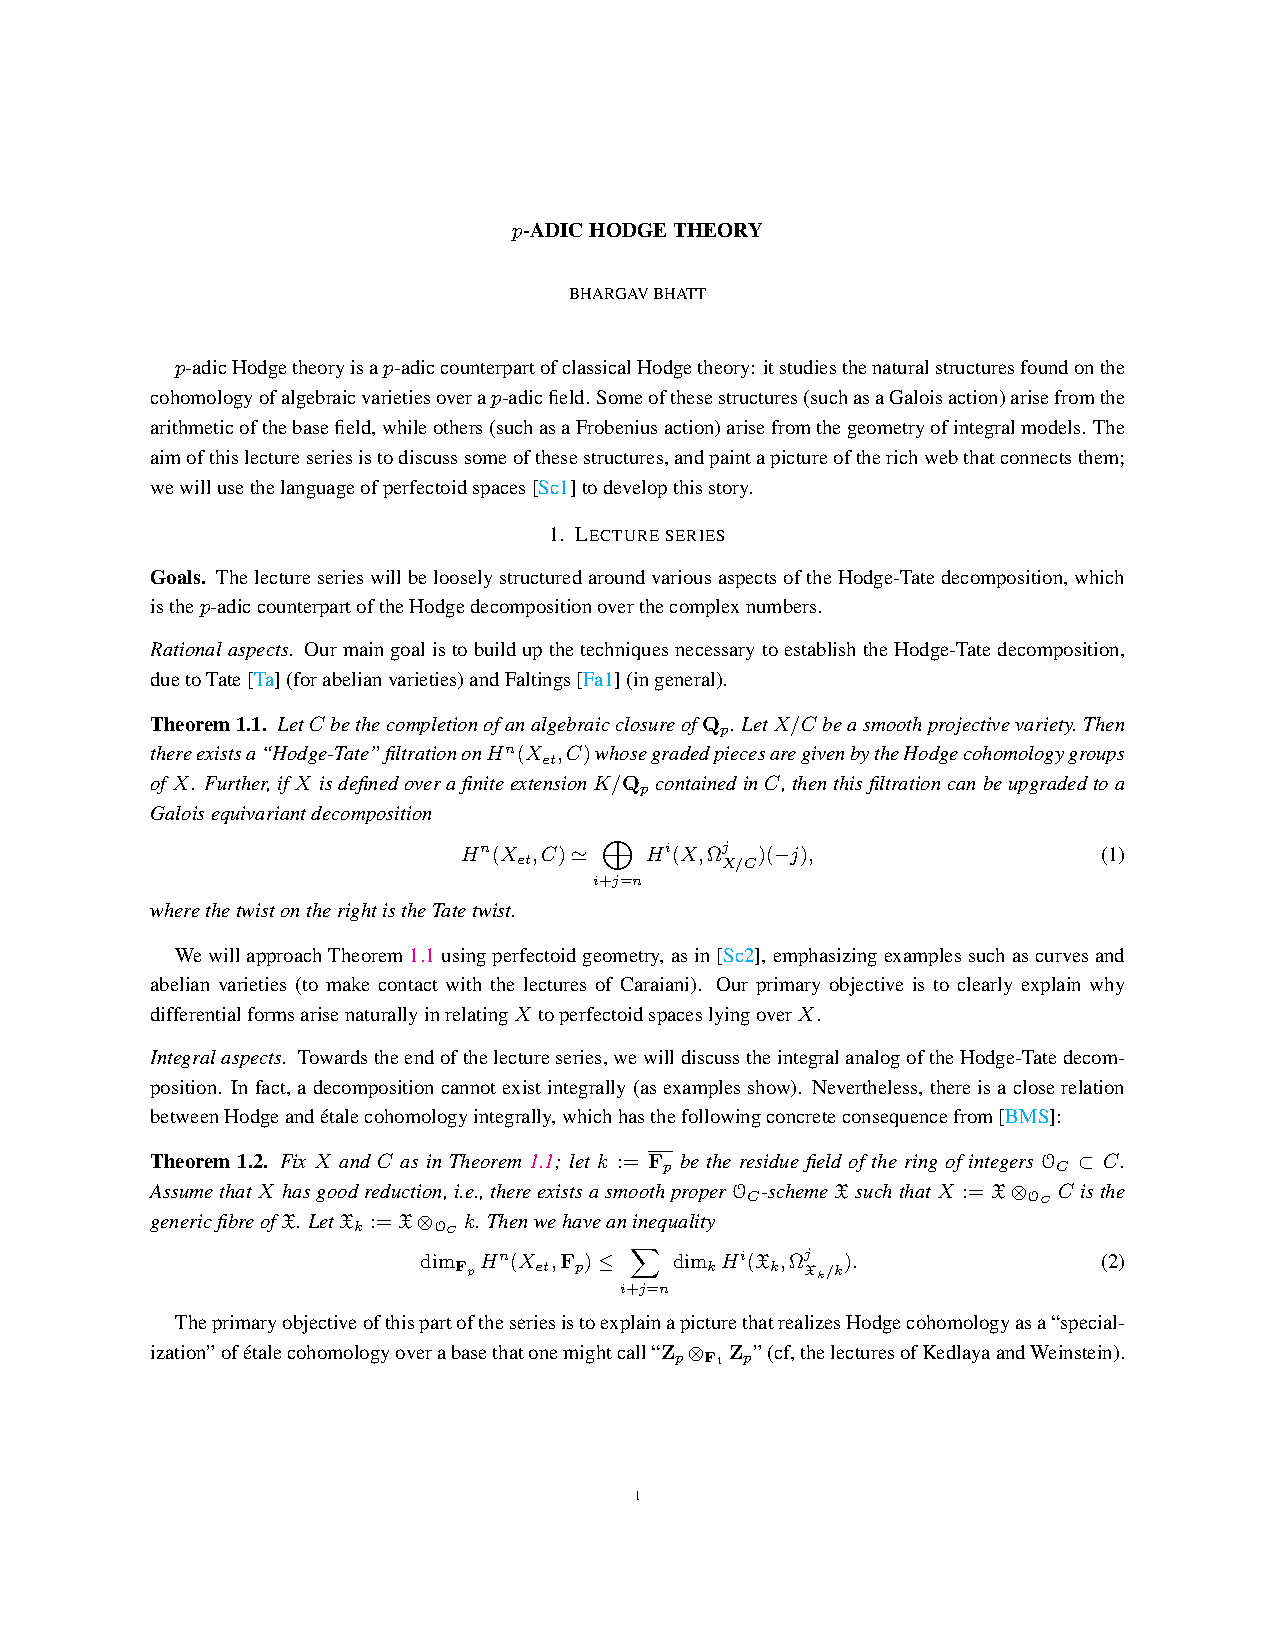
\includepdf[pages=-,scale=1,pagecommand={\thispagestyle{normal}}]{../notes/bhatt/2017BhattOutline.pdf}
\phantomsection
\addtocounter{subsection}{1}
\addcontentsline{toc}{subsection}{\protect\numberline{\thesubsection} Lecture Notes \& Project Description}

\includepdf[pages=-,scale=1,pagecommand={\thispagestyle{normal}}]{../notes/bhatt/2017BhattNotes.pdf}


% Caraiani
\phantomsection
\addtocounter{section}{1}
\addcontentsline{toc}{section}{\protect\numberline{\thesection} Ana Caraiani: Shimura Varieties}
\phantomsection
\setcounter{subsection}{1}
\addcontentsline{toc}{subsection}{\protect\numberline{\thesubsection} Course \& Project Outline}
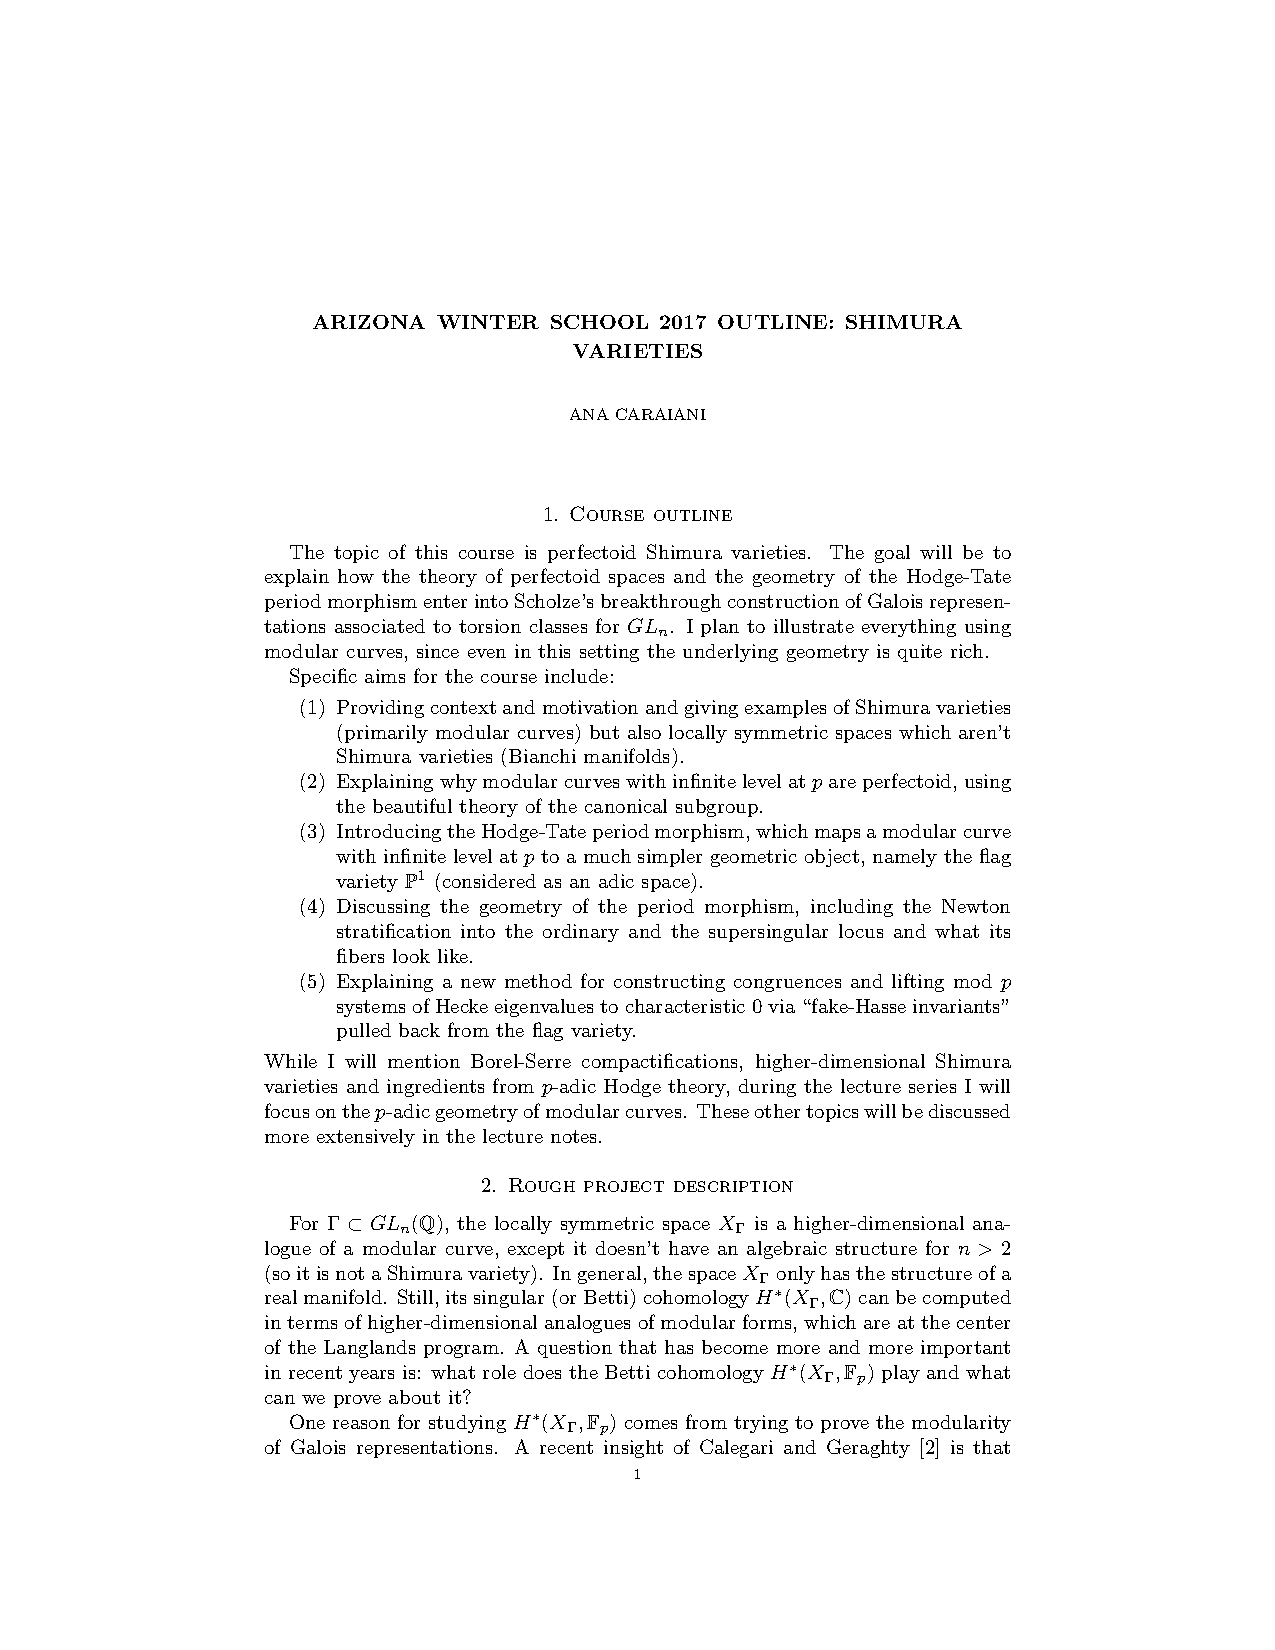
\includepdf[pages=-,scale=1,pagecommand={\thispagestyle{normal}}]{../notes/caraiani/2017CaraianiOutline.pdf}
\phantomsection
\addtocounter{subsection}{1}
\addcontentsline{toc}{subsection}{\protect\numberline{\thesubsection} Lecture Notes \& Project Description}
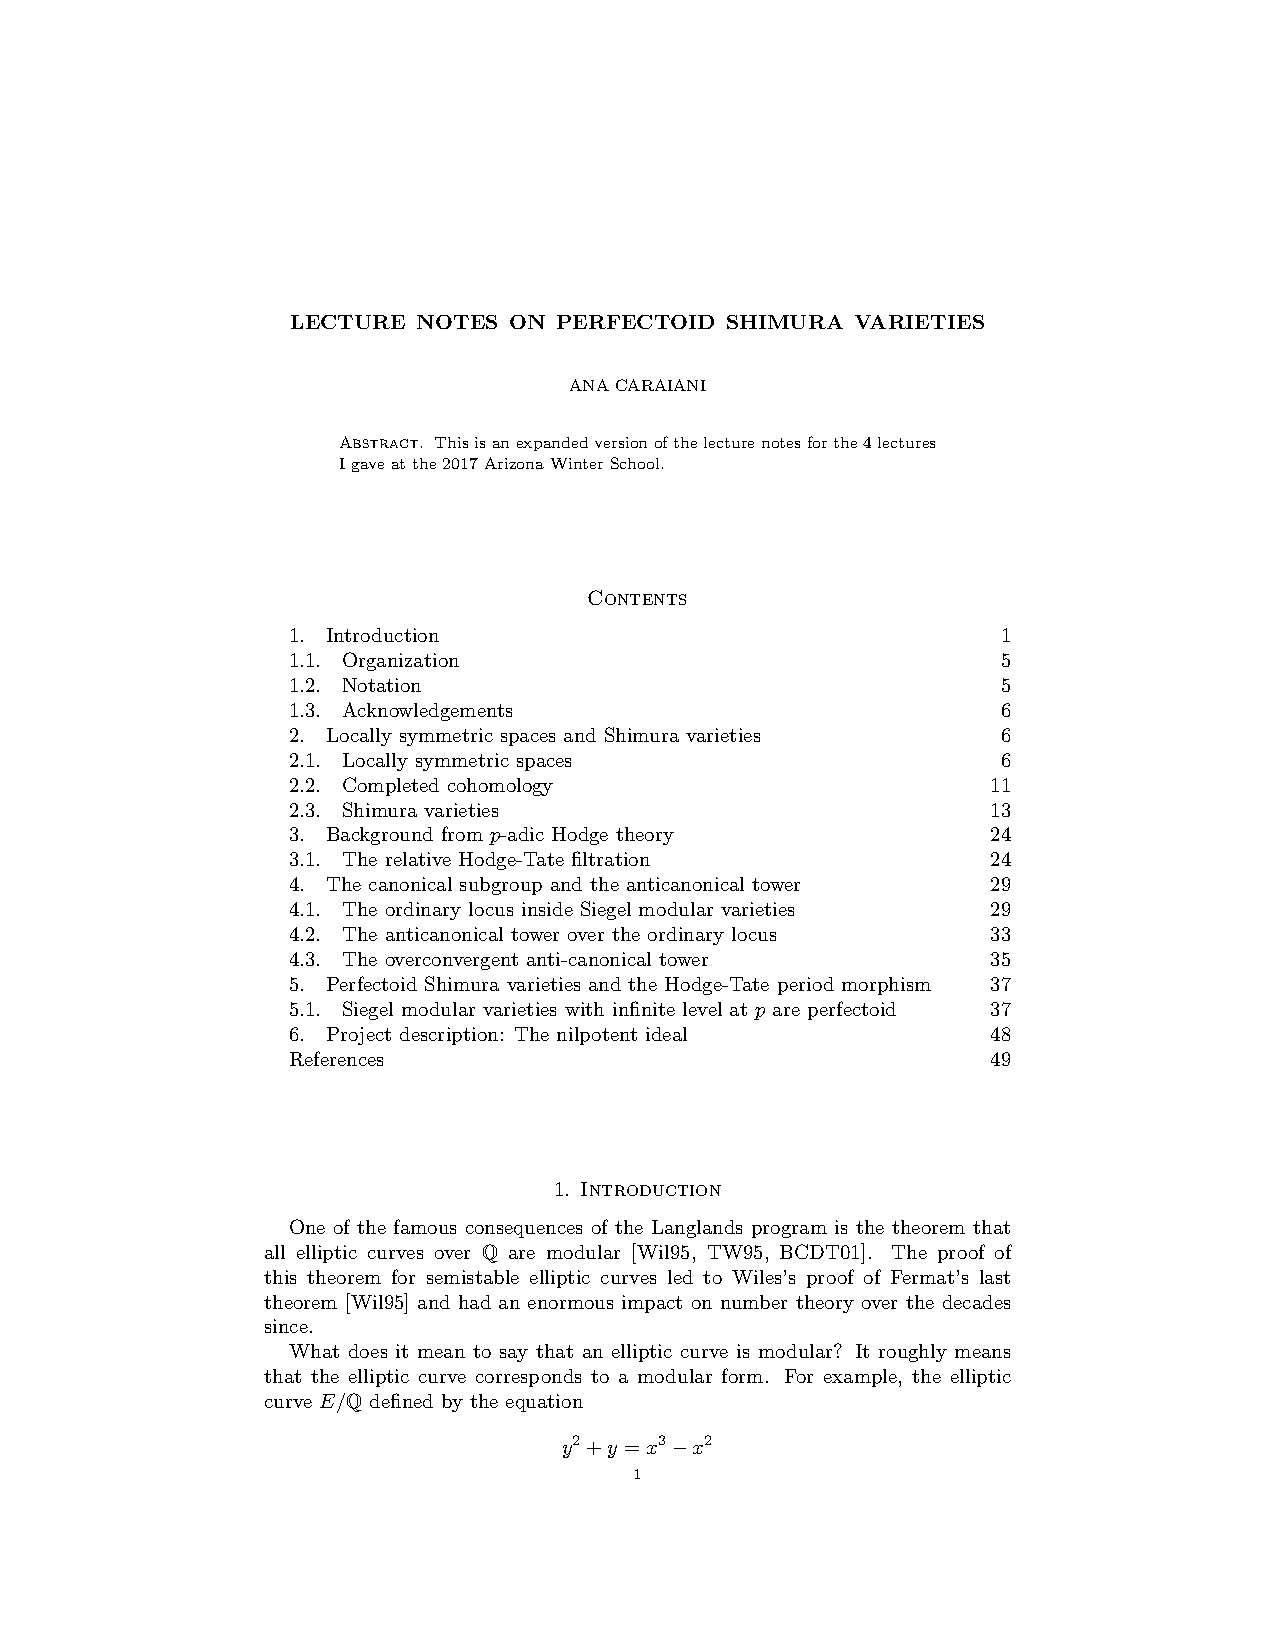
\includepdf[pages=-,scale=1,pagecommand={\thispagestyle{normal}}]{../notes/caraiani/2017CaraianiNotes.pdf}


% Kedlaya
\phantomsection
\addtocounter{section}{1}
\addcontentsline{toc}{section}{\protect\numberline{\thesection} Kiran Kedlaya: Sheaves, stacks, shtukas}
\phantomsection
\setcounter{subsection}{1}
\addcontentsline{toc}{subsection}{\protect\numberline{\thesubsection} Course \& Project Outline}
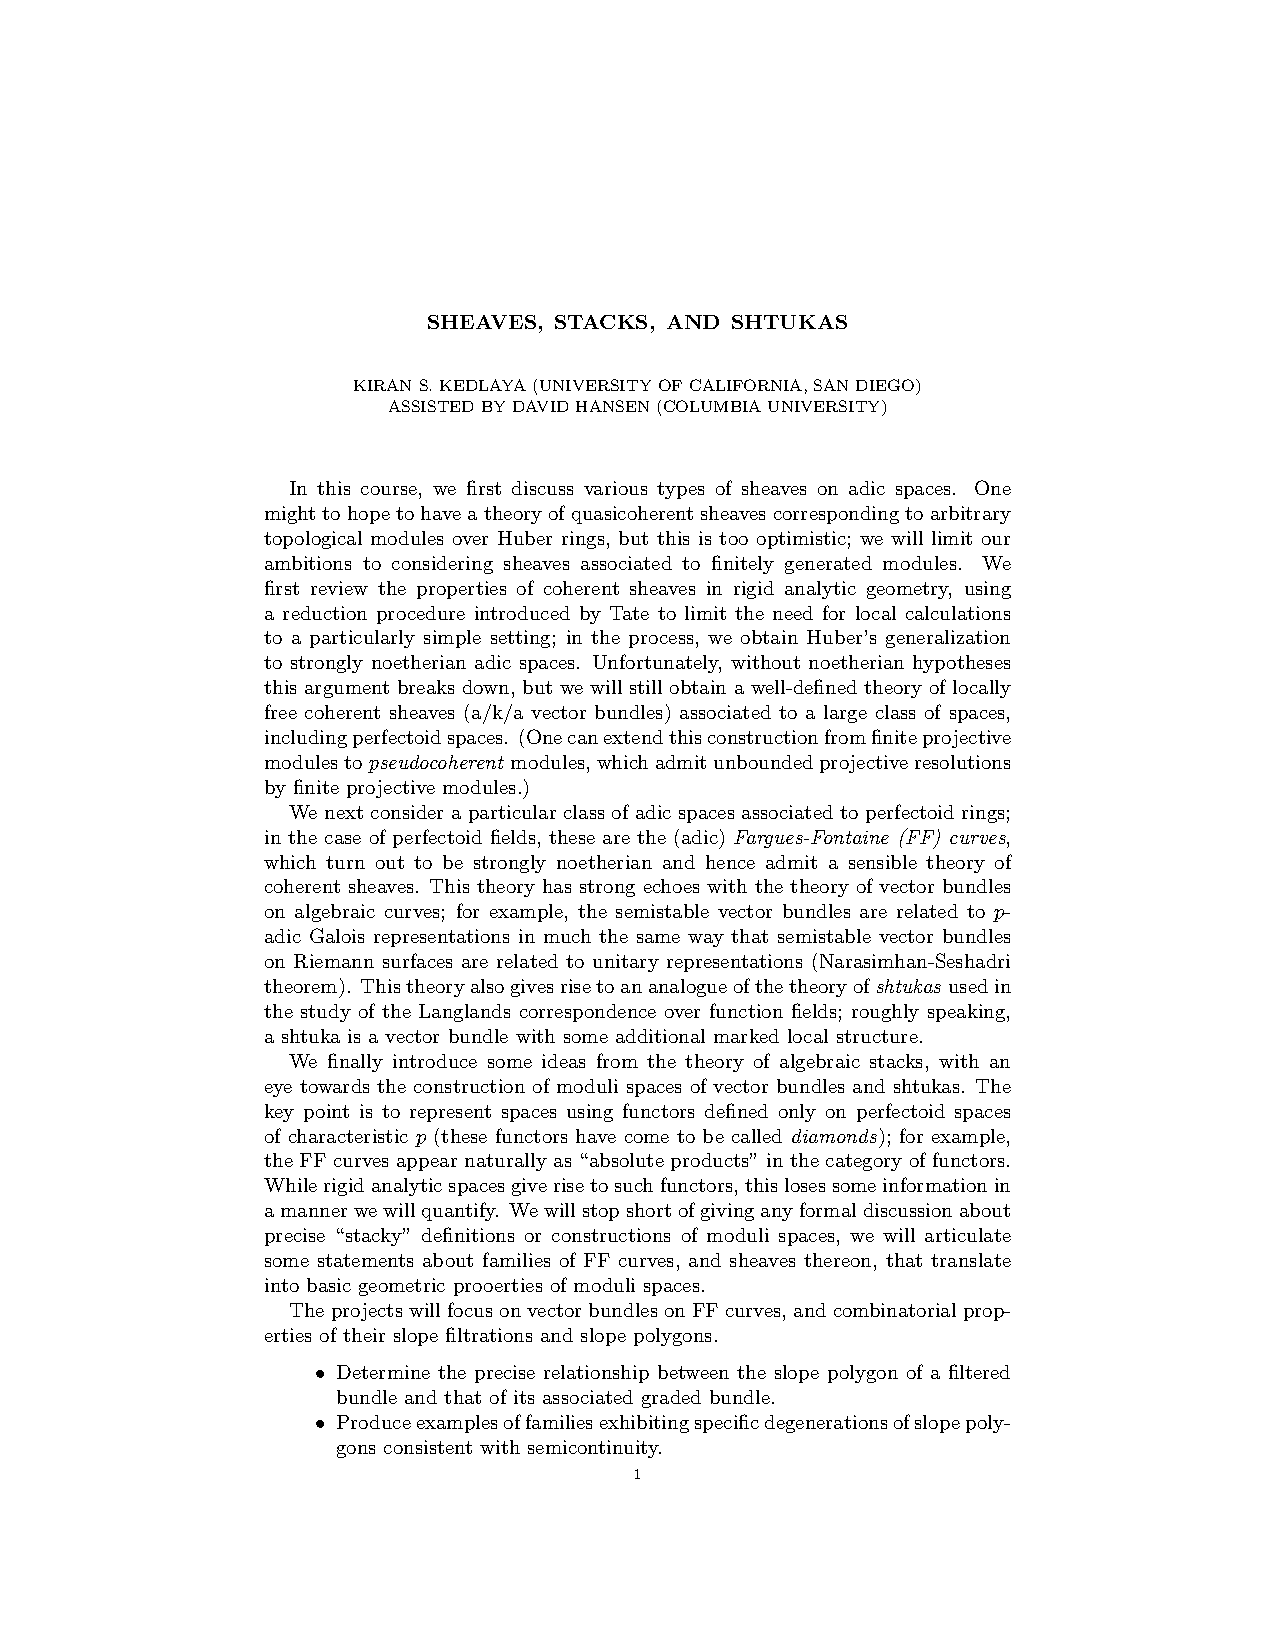
\includepdf[pages=-,scale=1,pagecommand={\thispagestyle{normal}}]{../notes/kedlaya/2017KedlayaOutline.pdf}
\phantomsection
\addtocounter{subsection}{1}
\addcontentsline{toc}{subsection}{\protect\numberline{\thesubsection} Lecture Notes \& Project Description}
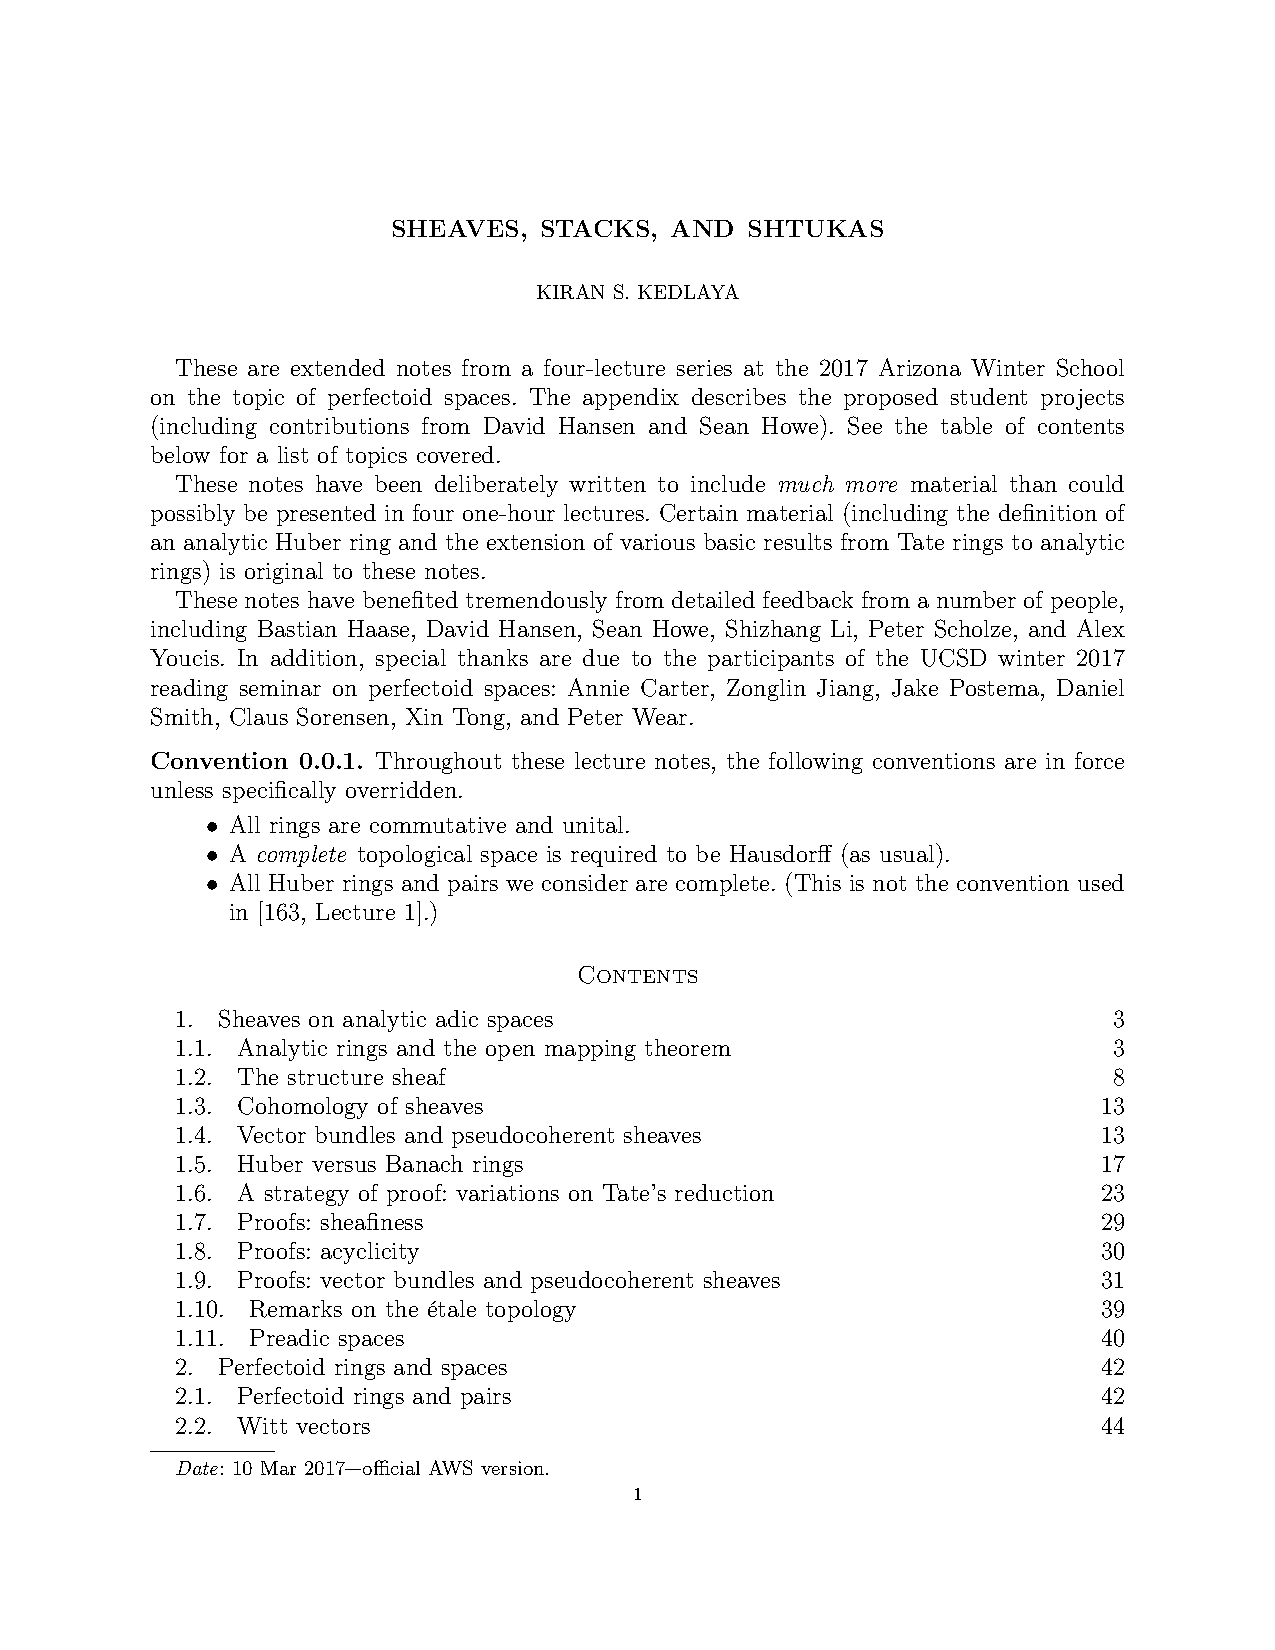
\includepdf[pages=-,scale=1,pagecommand={\thispagestyle{normal}}]{../notes/kedlaya/2017KedlayaNotes.pdf}


% Weinstein
\phantomsection
\addtocounter{section}{1}
\addcontentsline{toc}{section}{\protect\numberline{\thesection} Jared Weinstein: Adic spaces}
\phantomsection
\setcounter{subsection}{1}
\addcontentsline{toc}{subsection}{\protect\numberline{\thesubsection} Course \& Project Outline}
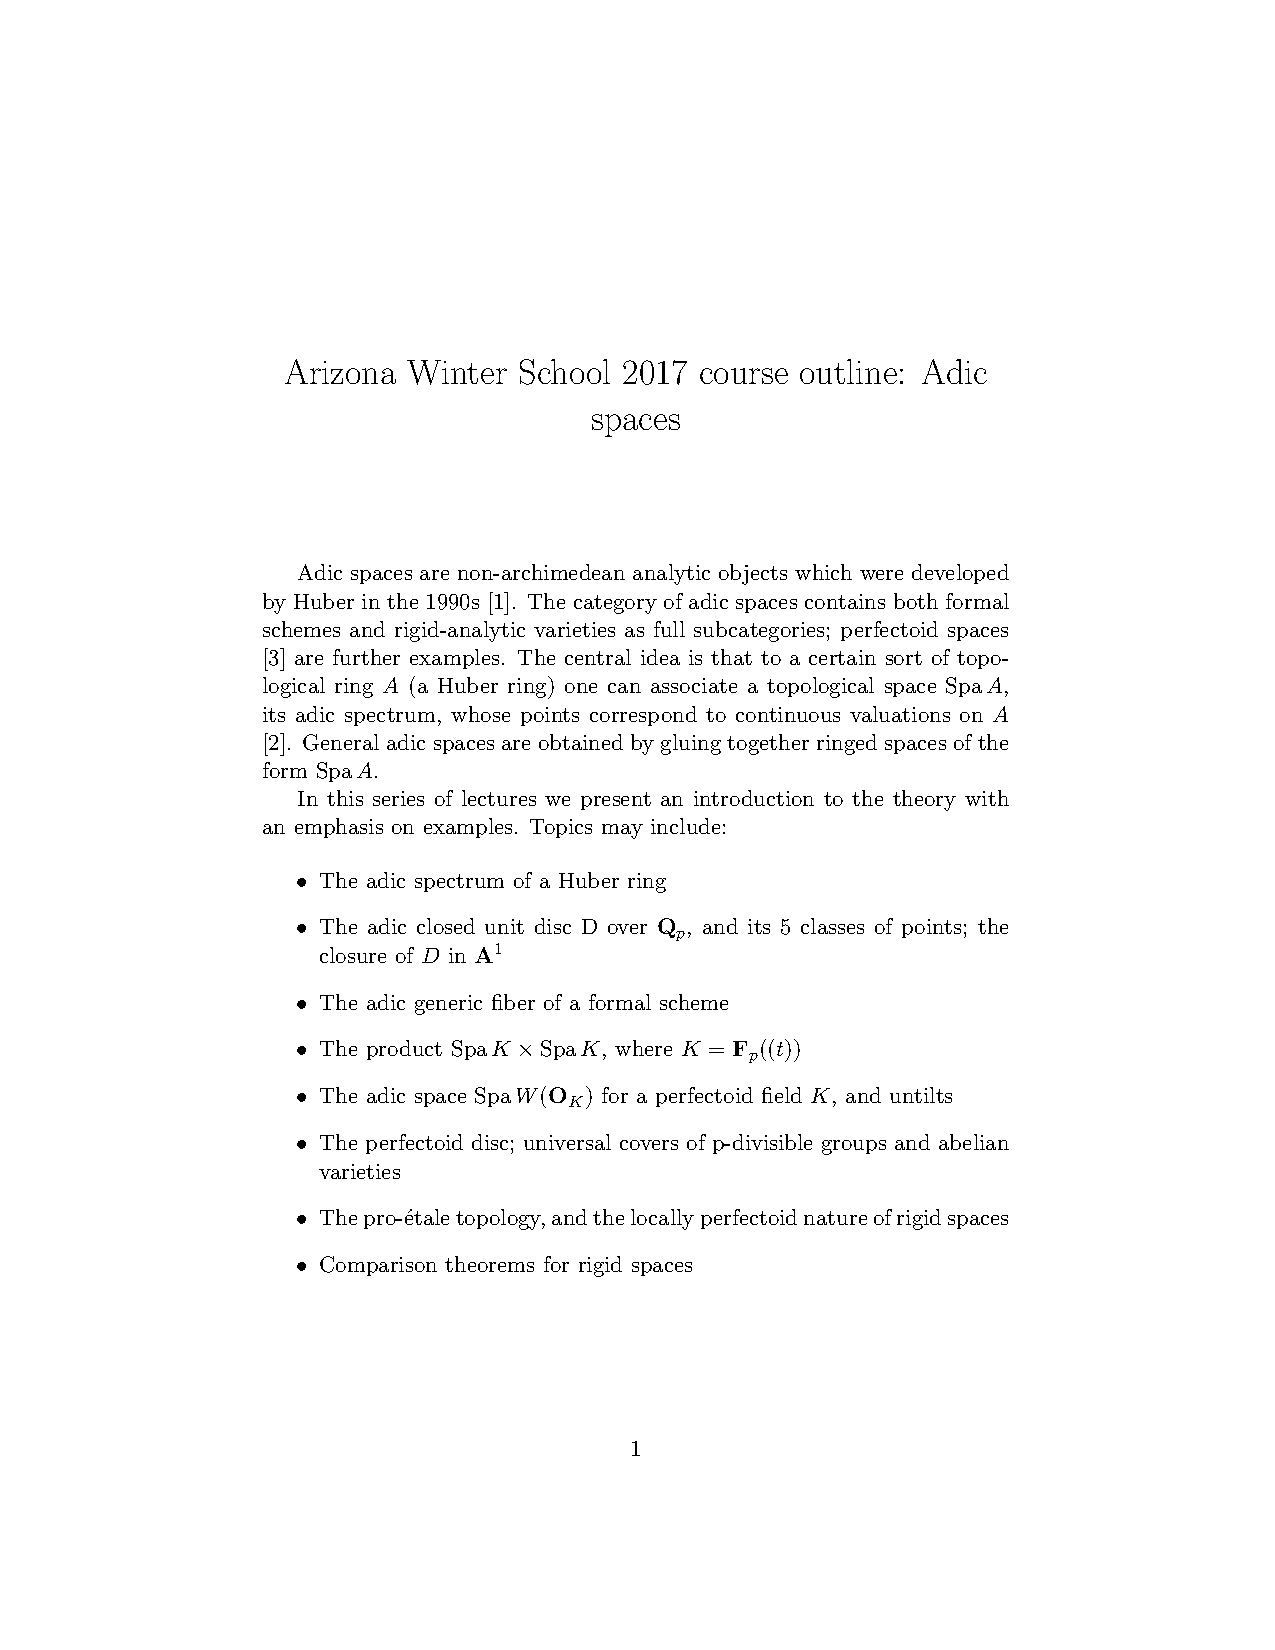
\includepdf[pages=-,scale=1,pagecommand={\thispagestyle{normal}}]{../notes/weinstein/2017WeinsteinOutline.pdf}
\phantomsection
\addtocounter{subsection}{1}
\addcontentsline{toc}{subsection}{\protect\numberline{\thesubsection} Lecture Notes \& Project Description}
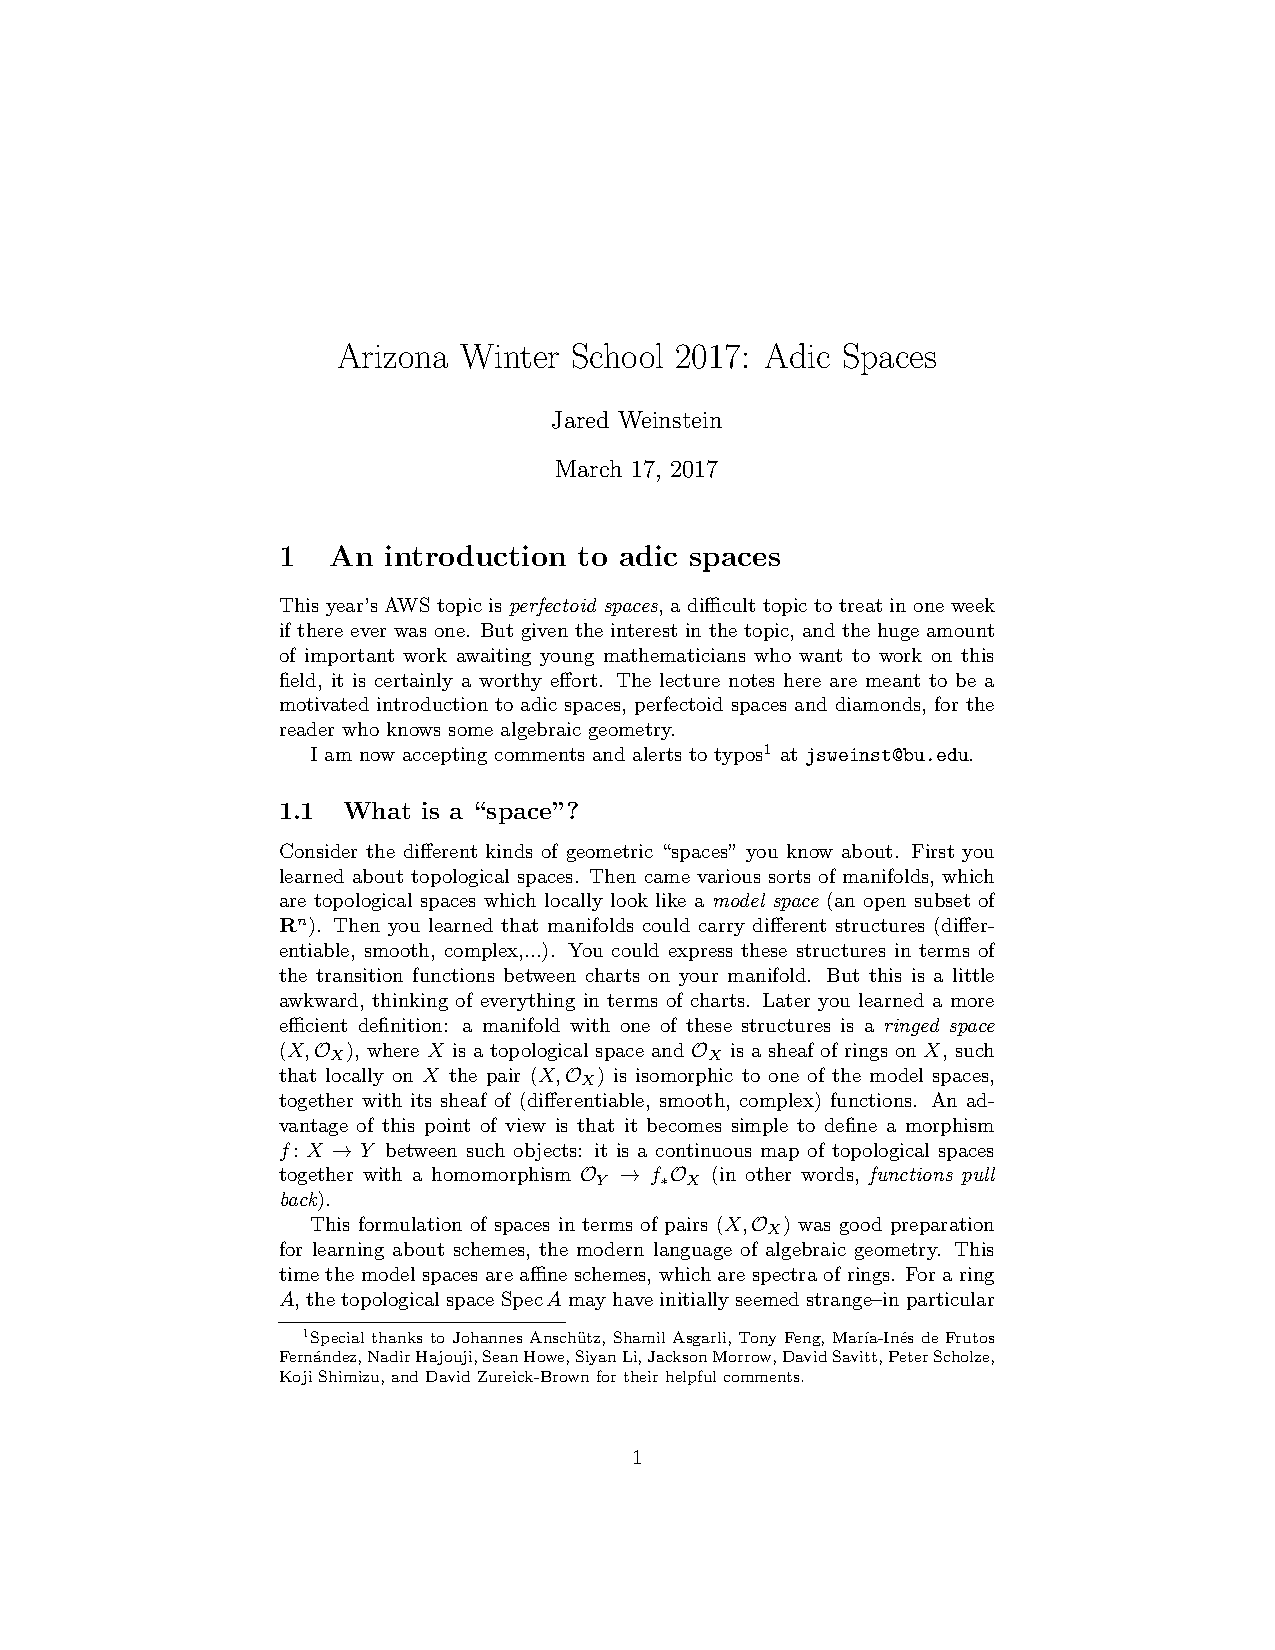
\includepdf[pages=-,scale=1,pagecommand={\thispagestyle{normal}}]{../notes/weinstein/2017WeinsteinNotes.pdf}


% Problem Groups
\phantomsection
\addtocounter{section}{1}
\addcontentsline{toc}{section}{\protect\numberline{\thesection} Problem Sessions}
\phantomsection
\setcounter{subsection}{1}
\addcontentsline{toc}{subsection}{\protect\numberline{\thesubsection} Yoichi Mieda: Adic spaces and perfectoid spaces}
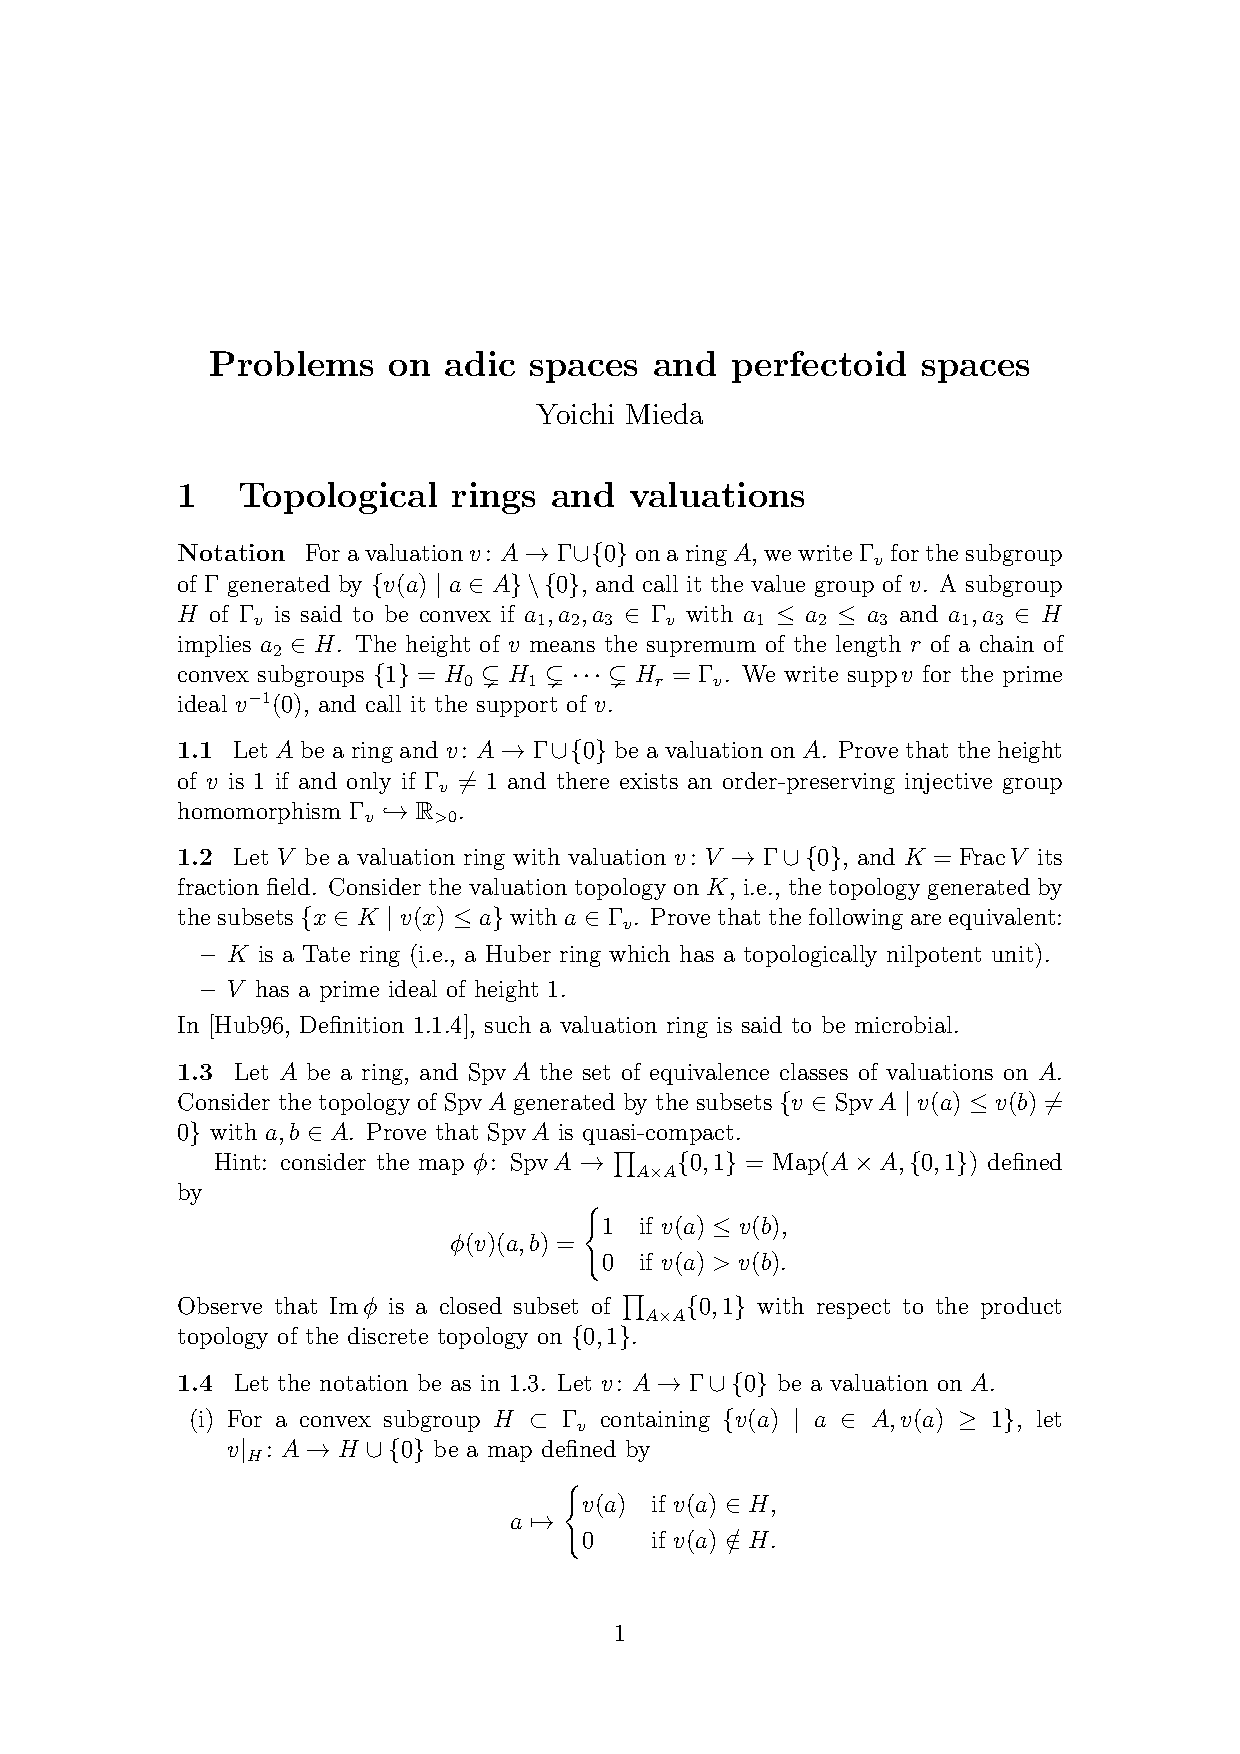
\includepdf[pages=-,scale=1,pagecommand={\thispagestyle{normal}}]{../notes/problem_groups/2017MiedaProblems.pdf}
\addcontentsline{toc}{subsection}{\protect\numberline{\thesubsection} Hansheng Diao: Period rings and period sheaves (abridged, no hints)}
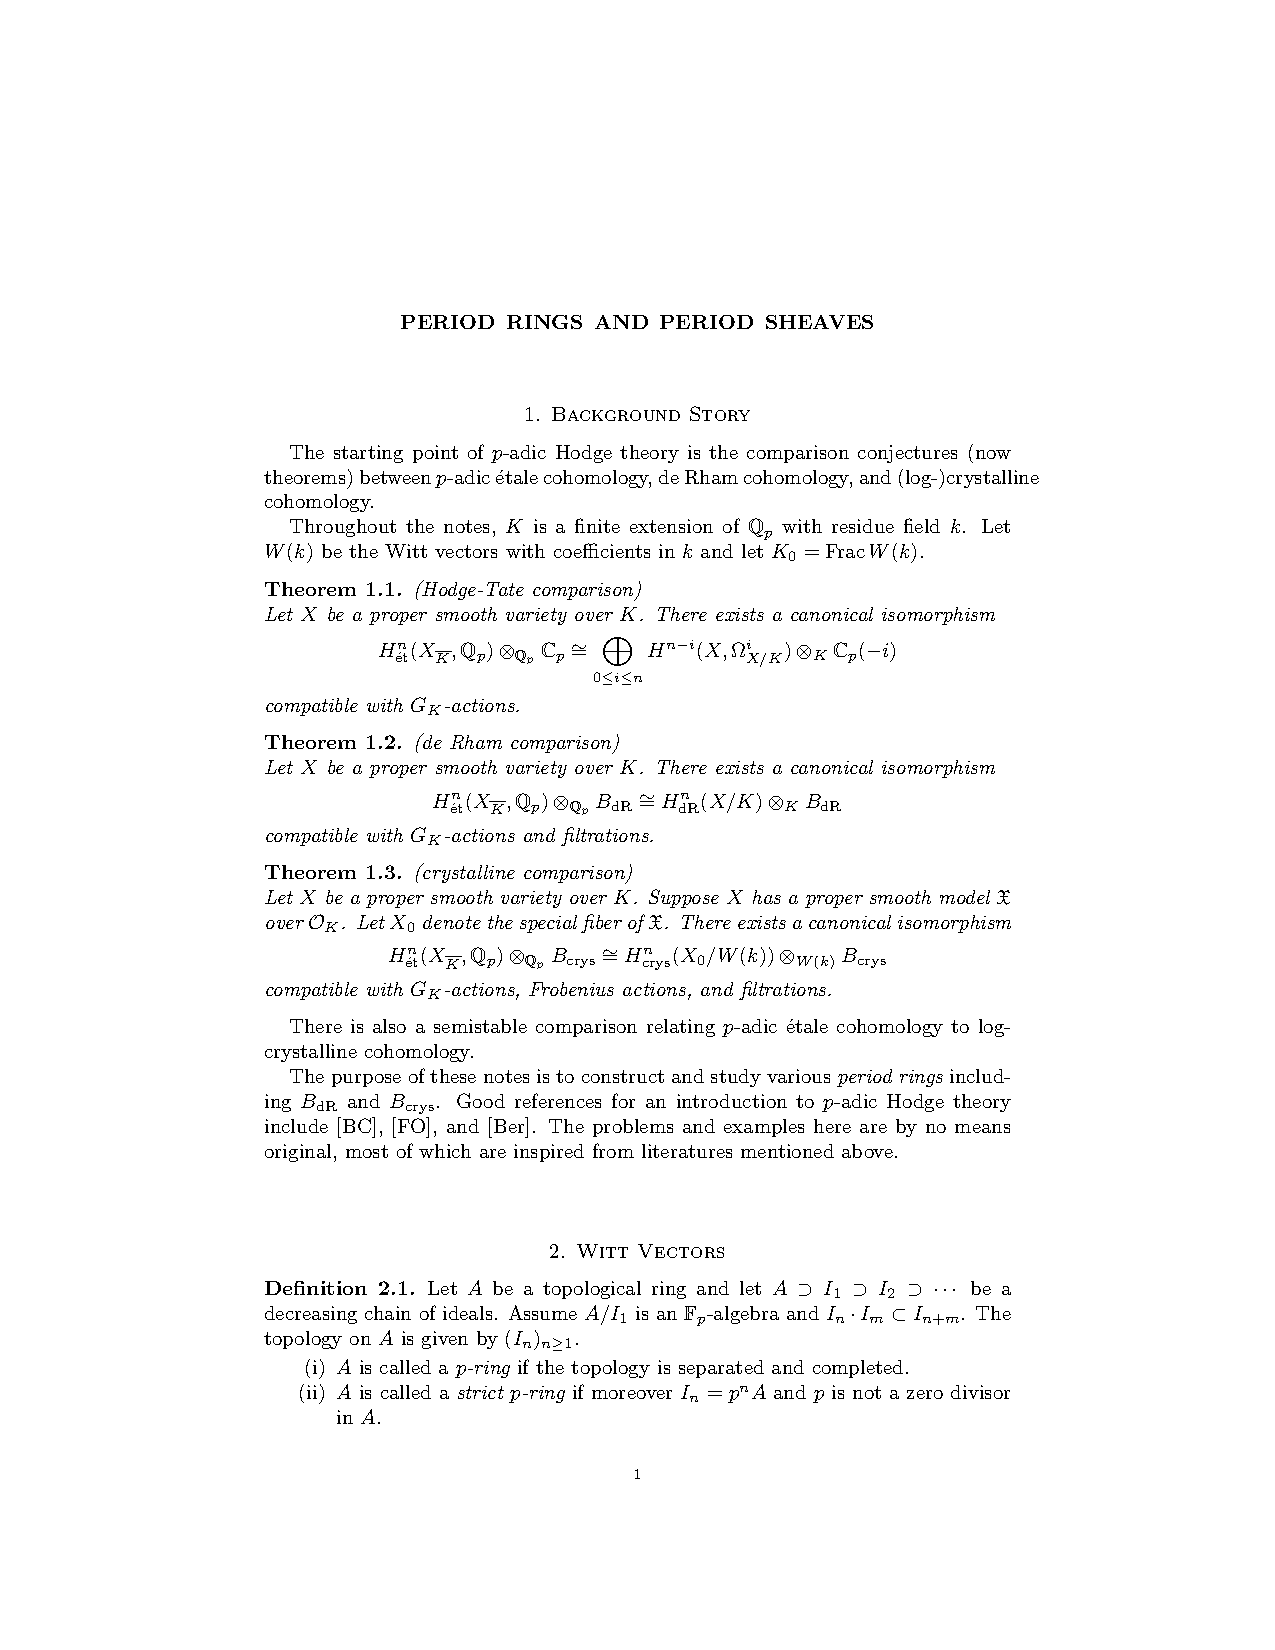
\includepdf[pages=-,scale=1,pagecommand={\thispagestyle{normal}}]{../notes/problem_groups/2017DiaoProblemsNH.pdf}
\addcontentsline{toc}{subsection}{\protect\numberline{\thesubsection} Hansheng Diao: Period rings and period sheaves (extended)}
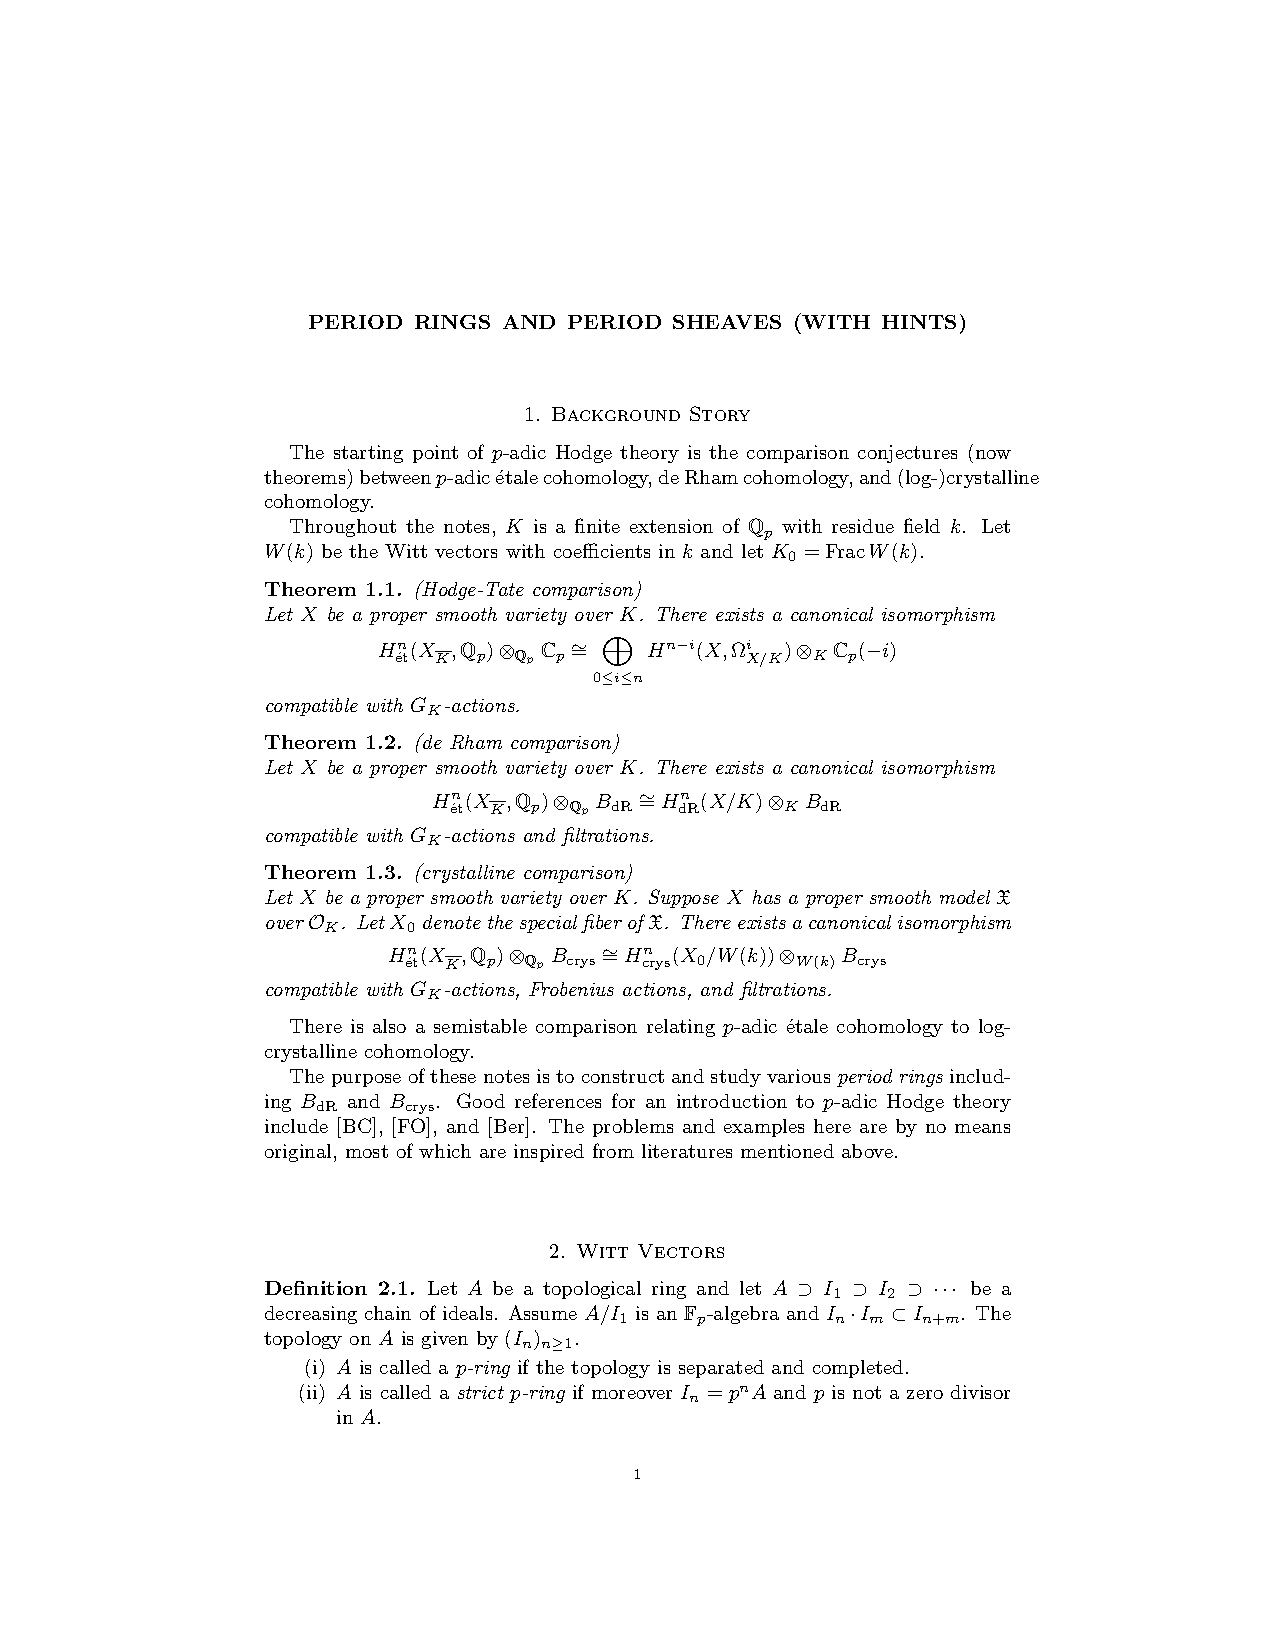
\includepdf[pages=-,scale=1,pagecommand={\thispagestyle{normal}}]{../notes/problem_groups/2017DiaoProblems.pdf}
}


% -------------------
% Bibliography
% -------------------
\newpage
\nocite{*}
\printbibliography

\end{document}